

\documentclass[english]{beamer}
\usepackage{mathptmx}
\usepackage[T1]{fontenc}
\usepackage[latin9]{inputenc}
\usepackage{url}
\usepackage{amsmath}
\usepackage{amssymb}
\usepackage{graphicx}
\usepackage{mathtools}
\usepackage{dsfont}
\usepackage{hyperref}

\makeatletter
\newcommand\makebeamertitle{\frame{\maketitle}}%
\AtBeginDocument{%
  \let\origtableofcontents=\tableofcontents
  \def\tableofcontents{\@ifnextchar[{\origtableofcontents}{\gobbletableofcontents}}
  \def\gobbletableofcontents#1{\origtableofcontents}
}
\setbeamertemplate{navigation symbols}{%
    \usebeamerfont{footline}%
    \usebeamercolor[fg]{footline}%
    \hspace{1em}
}

\definecolor{blue(pigment)}{rgb}{0.2, 0.2, 0.6}


\setbeamercolor{footline}{fg=black}
\setbeamerfont{footline}{series=\bfseries}
\setbeamercolor{frametitle}{fg=blue(pigment)}
\setlength{\leftmargini}{5pt}

\usepackage{lmodern}

\makeatother

\usepackage{babel}

 
\begin{document}

\title{\textcolor{blue(pigment)}{Text Analysis for Economics and Finance}}
\vspace{8pt} 
\author{Ruben Durante\\
\small{ICREA-UPF, BGSE, IPEG, CEPR}}
\date{\small{DIW, October 2020}}

\frame{\titlepage}
\setbeamercovered{dynamic}
%%%%%%%%%%%%%%
\begin{frame}{Generative methods}
\begin{itemize}
\setlength{\itemsep}{1.3em}
    \item \textcolor{blue}{``Supervised'' methods:} pursuing a known goal
    \begin{itemize}
        \item i.e. predicting authorship of an academic paper
    \end{itemize}
    \item \textcolor{blue}{``Unsupervised'' methods:} pursuing an unknown goal 
    \begin{itemize}
        \item algorithm is tasked with discovering patterns and themes in data
    \end{itemize}
    \pause
    \item Both transform high-dimensional data into low-dimensional measures, preserving as much variation as possible
    \vspace{3pt}
    \begin{itemize}
    \setlength{\itemsep}{0.4em}
        \item Congressional roll call votes $\rightarrow$ ``common space'' scores
        \item Survey responses $\rightarrow$ ``Big 5'' personality traits
    \end{itemize}
   \pause
    \item Low dimensional measures are then used as inputs in analysis
        \vspace{3pt}
    \begin{itemize}
        \setlength{\itemsep}{0.4em}
        \item How has polarization in Congress changed over time?\\(Poole-Rosenthal 1984)
        \item How does personality correlate with job performance? (Tett et al. 1991)
    \end{itemize}
    \end{itemize}
\end{frame}
%%%%%%%%%%%%%%
\begin{frame}{Topic models}
\begin{itemize}
\setlength{\itemsep}{0.8em}
    \item Topic models extend factor models (e.g., PCA) to multinomial data like text
    \item Topic models are based on the idea that documents are \textcolor{blue}{mixtures of topics}, where a topic is a probability distribution over words
\item A topic model is a generative model for documents: it specifies a simple probabilistic process by which documents are generated
\pause
    \item Relevant to measuring, e.g.:
     \vspace{7pt}
    \begin{itemize}
    \setlength{\itemsep}{0.8em}
        \item What people talk about on social networks?
        \item What products share similar descriptions on Amazon or EBay?
        \item What stories are in the news today?
        \item What are economists studying?
    \end{itemize}
\end{itemize}
\end{frame}
%%%%%%%%%%%%%%
\begin{frame}{Blei-Lafferty, 2006: how did ``Science'' change over time?}
\centering

\includegraphics[width = .35 \textwidth]{Images/science.png}
\vspace{5pt}
\pause
\begin{itemize}
    \item OCR text of \textit{Science} 1880-2002 (from JSTOR, full text)
     \vspace{5pt}
    \begin{itemize}
        \setlength{\itemsep}{0.5em}
        \item Count words used 25 or more times (after stemming, stopwords removal)
        \item Vocabulary: 15,955 words
        \item Total documents: 30,000 articles
    \end{itemize}
\end{itemize}
\end{frame}
%%%%%%%%%%%%%%
\begin{frame}{What does this method produce?}
\begin{center}
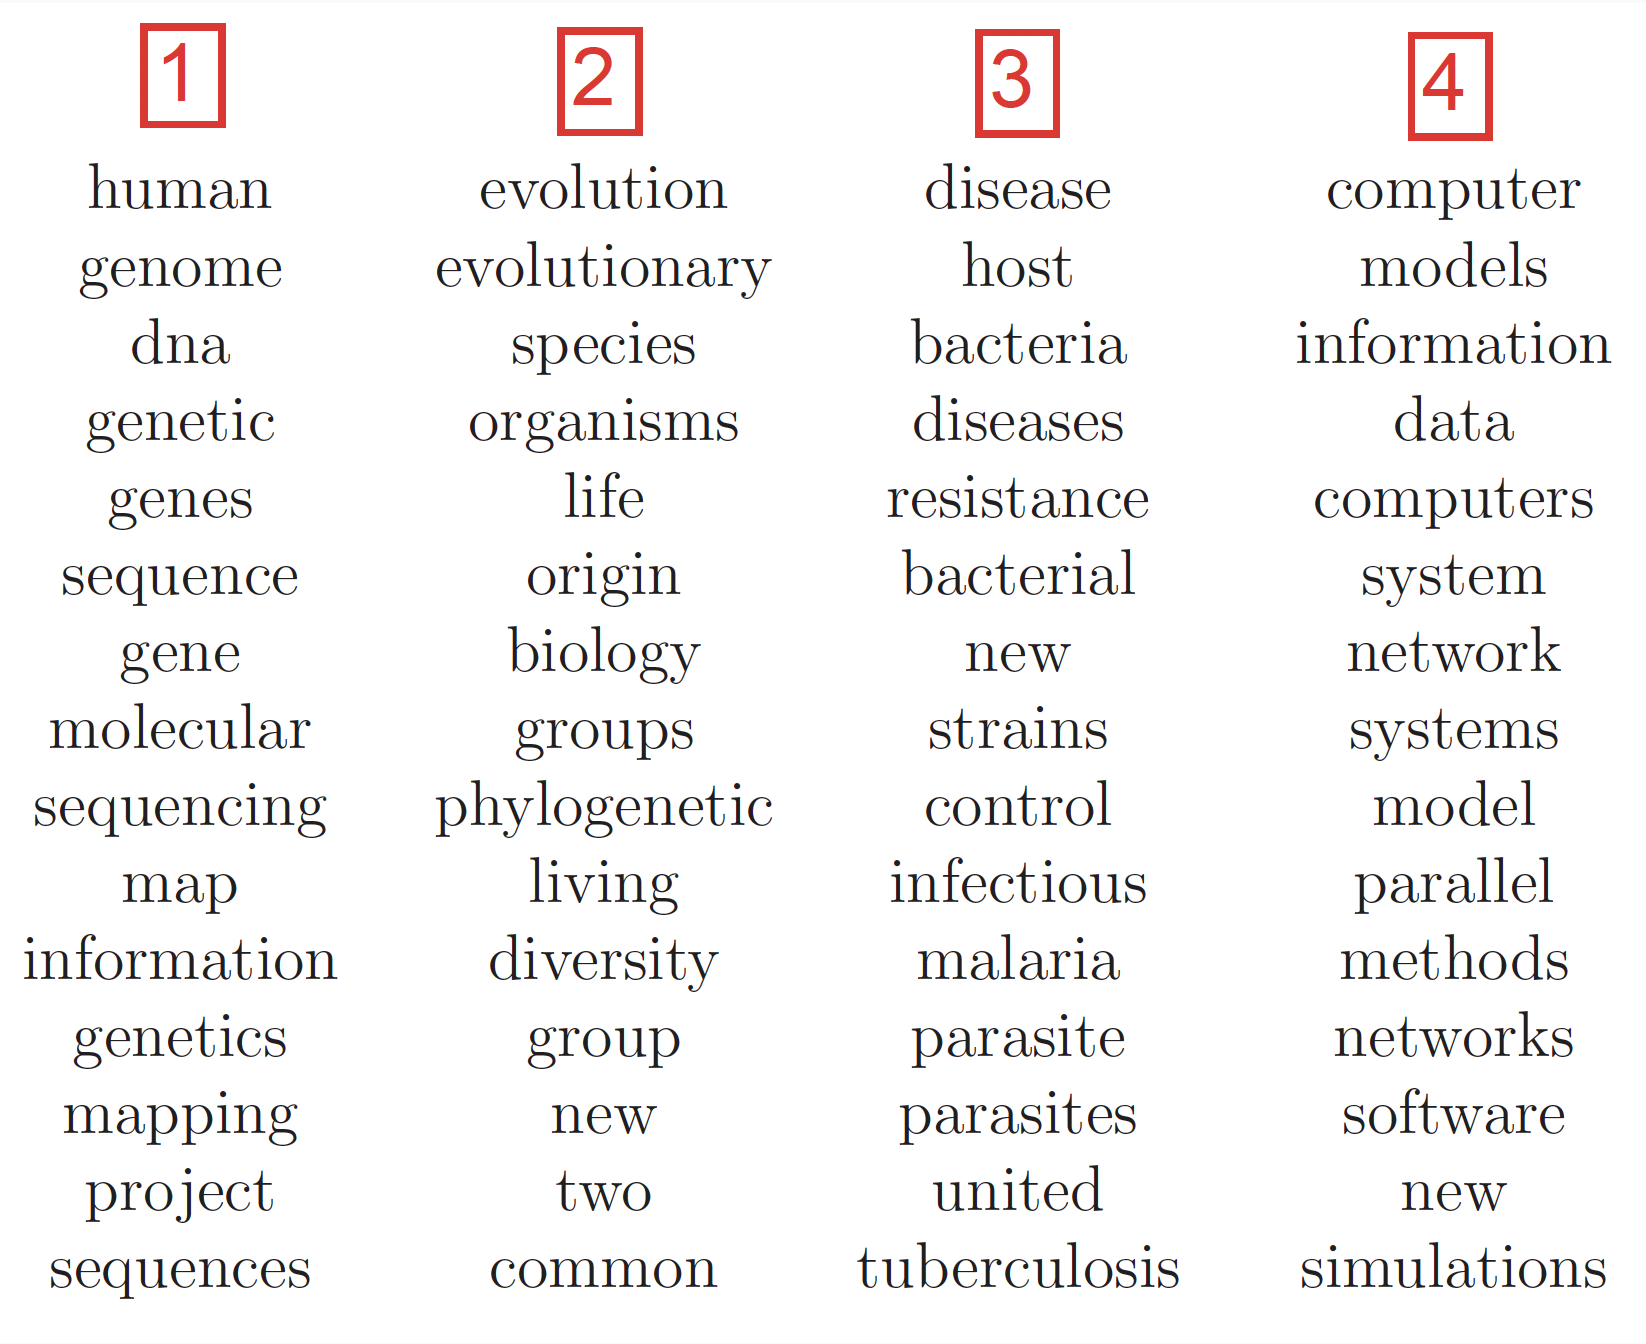
\includegraphics[width=0.9 \textwidth]{Images/topics_output.png}
\end{center}
\end{frame}
%%%%%%%%%%%%%%
\begin{frame}{What does this method produce? (cont.)}
\centering
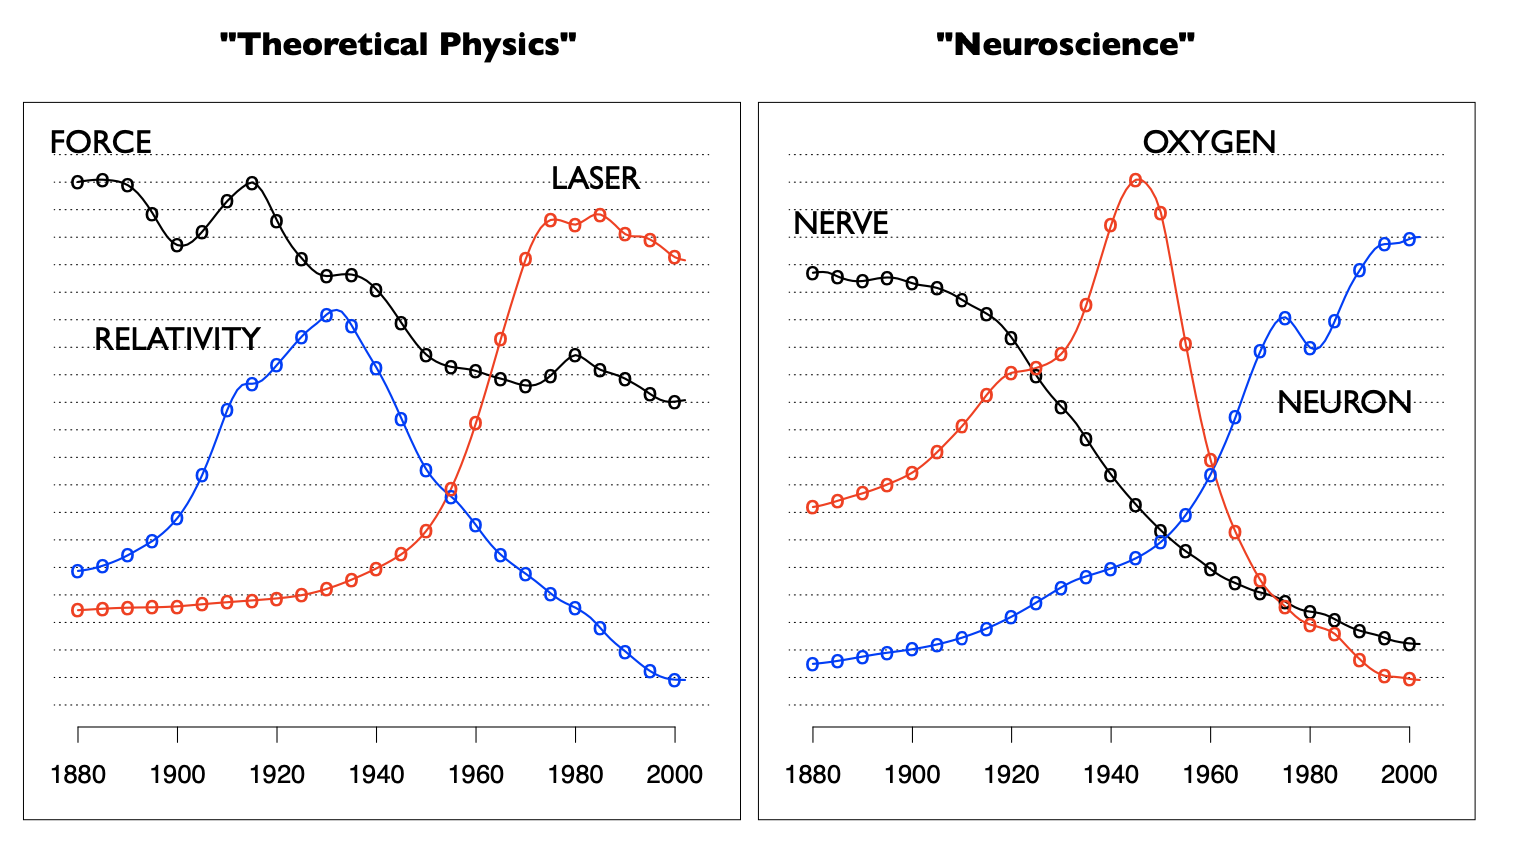
\includegraphics[width=1 \textwidth]{Images/plots.png}    
\end{frame}
%%%%%%%%%%%%%%
\begin{frame}{Model: LDA}
\begin{itemize}
        \setlength{\itemsep}{1.2em}
    \item Latent Dirichlet Allocation (LDA) extends of factor models to discrete data
\item  LDA : generative probabilistic model that assumes each topic is a mixture over an underlying set of words, and each document is a mixture of over a set of topic probabilities.
\end{itemize}
\end{frame}
%%%%%%%%%%%%%%
\begin{frame}{Model: LDA}
\begin{itemize}
        \setlength{\itemsep}{0.6em}
    \item Setup:
    \vspace{4pt}
    \begin{itemize}
            \setlength{\itemsep}{0.3em}
        \item Documents $i \in \{1,..., n\}$
        \item Words $j \in \{1,..., p\}$
        \item Data $\textbf{x}_i$ is a $(1 \times p)$ vector of word counts for document $i$
    \end{itemize}
\pause
\item Factor model:
    \vspace{4pt}
    \begin{itemize}
            \setlength{\itemsep}{0.3em}
        \item $\theta_{ik}$ is value of $k$-th \textbf{factor} for document $i$
        \item $\beta_k$ if $(1 \times p)$ vector of \textbf{loadings} for factor $k$
    \end{itemize}
        \begin{center}
        $E(x_i) = \beta_1 \theta_{i1} + ... + \beta_k \theta_{ik}$
        \end{center}
        
        \vspace{-8pt}
        
\pause
\item LDA:
    \vspace{4pt}
    \begin{itemize}
            \setlength{\itemsep}{0.3em}
        \item $\theta_{ik}$ is weight on $k$-th \textbf{topic} for document $i$ 
        \item $\beta_k$ is a $(1 \times p) $ vector of \textbf{word probabilities} for topic $k$
    \end{itemize}
    \begin{center}
        $\textbf{x}_i \sim Multinomial (\beta_1 \theta_{i1} + ... + \beta_k \theta{ik})$
    \end{center}
\end{itemize}
\end{frame}
%%%%%%%%%%%%%%
\begin{frame}{Model: LDA}
\centering
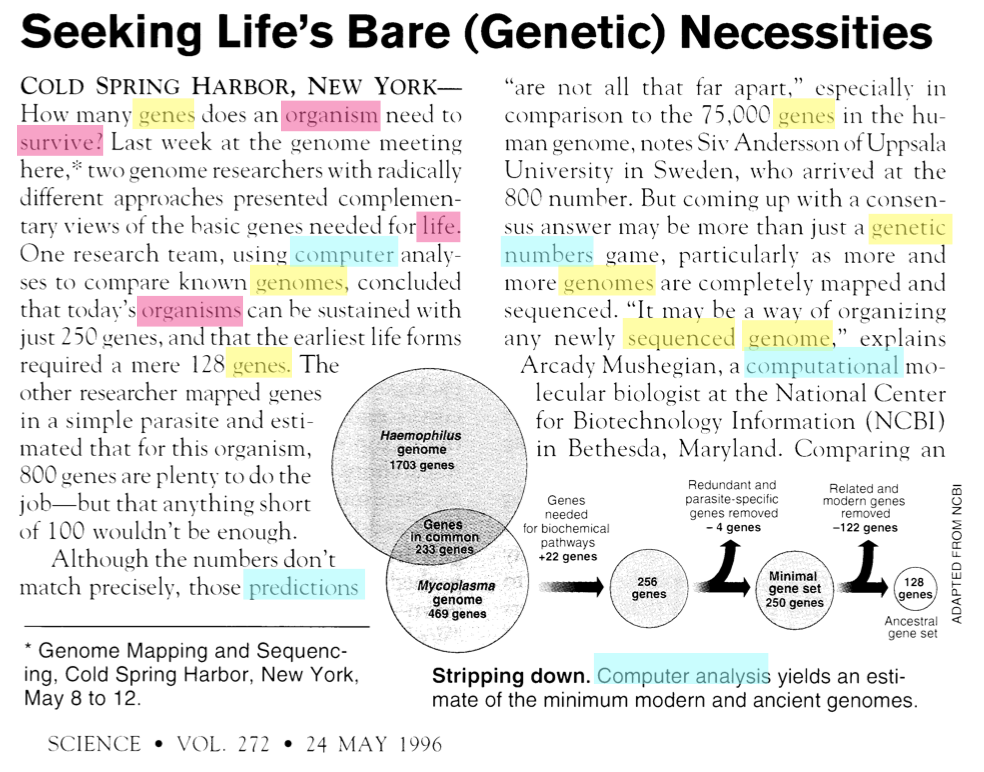
\includegraphics[width=0.85 \textwidth]{Images/page.png}
\begin{itemize}
\item \textcolor{blue}{Important}: each article can be about multiple topics (mixture)
\end{itemize}
\end{frame}
%%%%%%%%%%%%%%
\begin{frame}{Model: LDA}
\centering
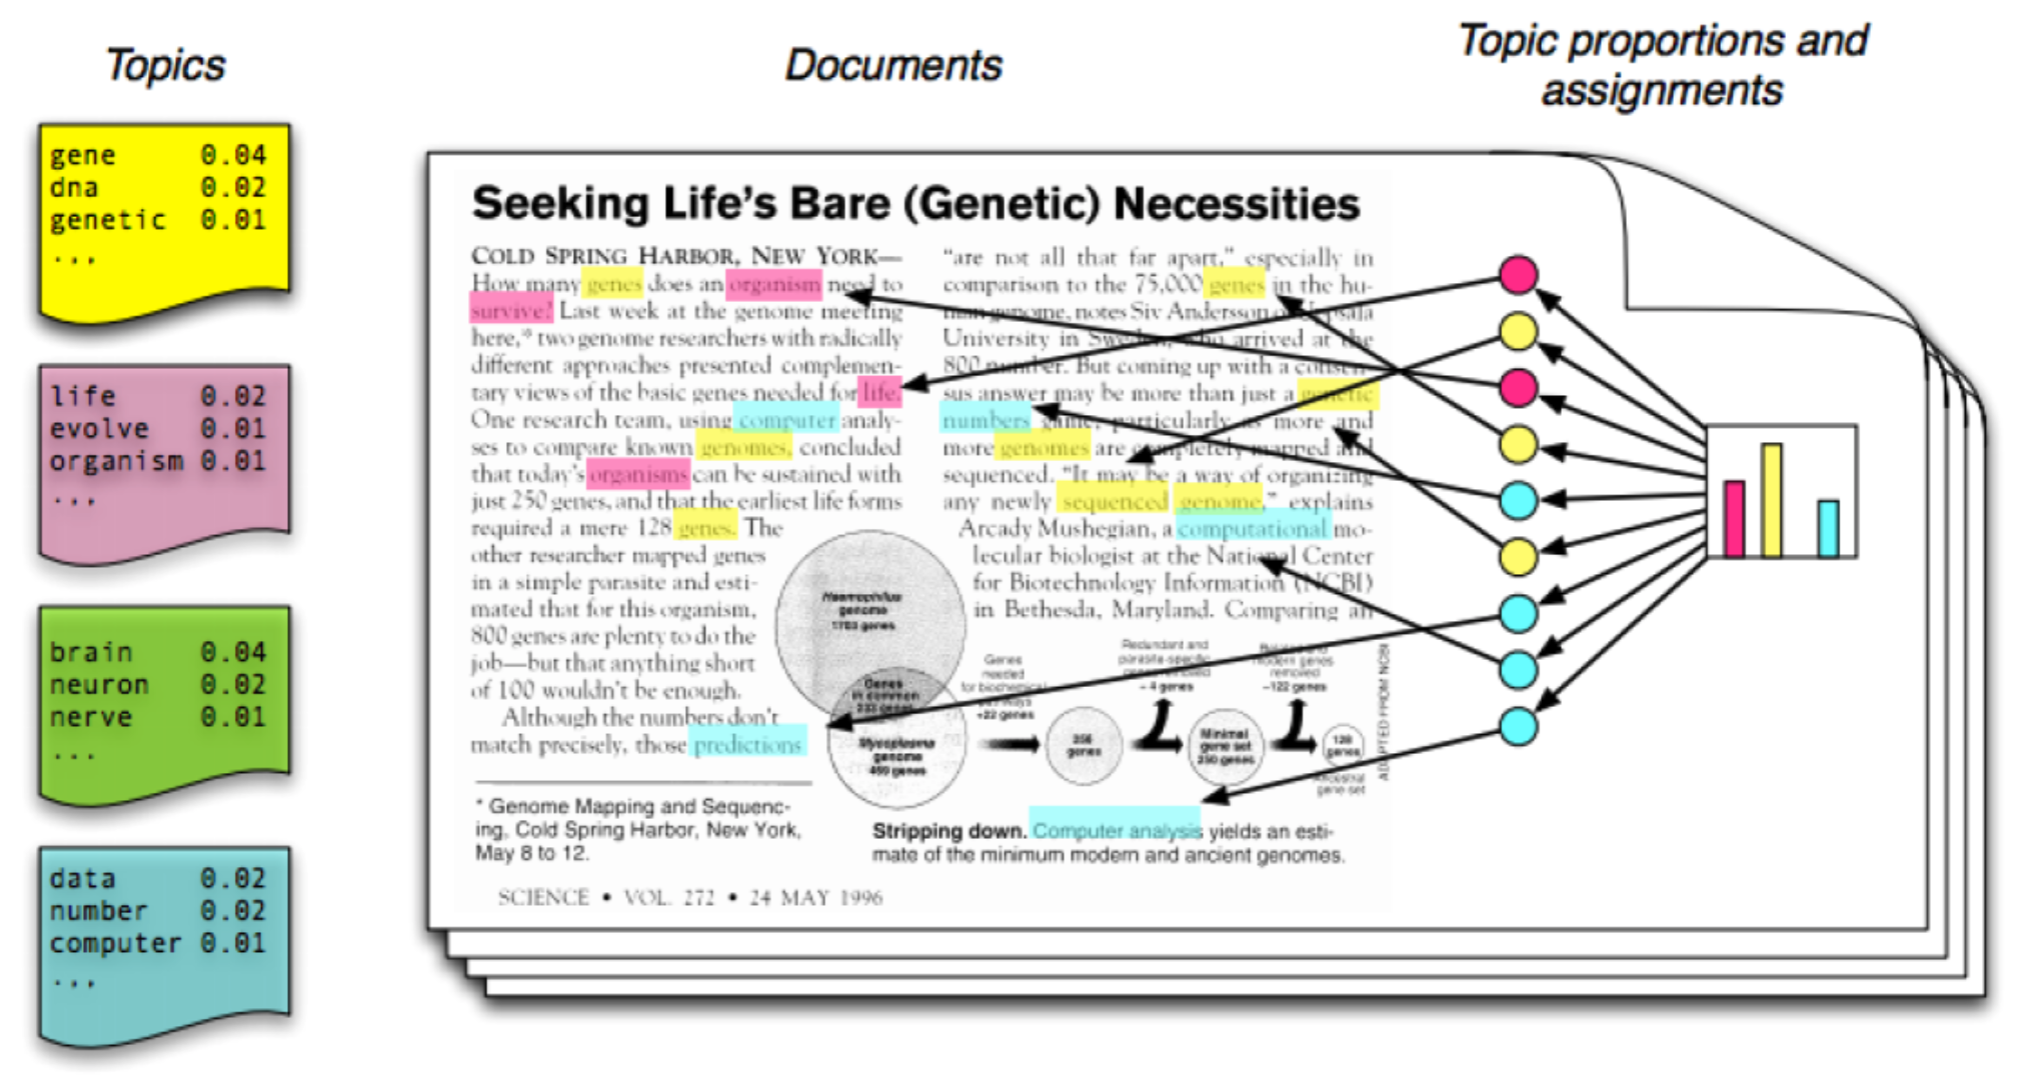
\includegraphics[width=1 \textwidth]{Images/page2.png}
\begin{itemize}
\item The weights, in turn, determine the probability of different words within that document 
\end{itemize}
\end{frame}
%%%%%%%%%%%%%%
\begin{frame}{Model: LDA}
\centering
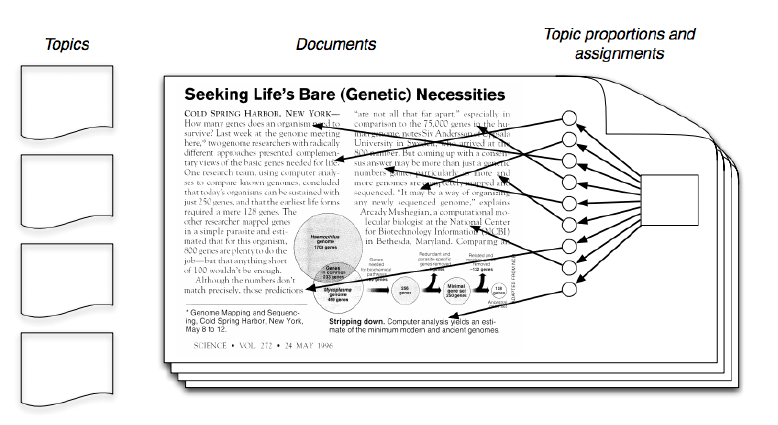
\includegraphics[width=0.8 \textwidth]{Images/blei2.png}
\begin{itemize}
\setlength{\itemsep}{1em}
    \item We don't observe the parameters of the model: we only observe documents and associated word count vectors, the remaining structure are hidden variables
    \item Conditional on the observed documents or word counts, we want to infer the parameters of the multinomials
\end{itemize}
\end{frame}
%%%%%%%%%%%%%
\begin{frame}{Model: LDA}
\centering
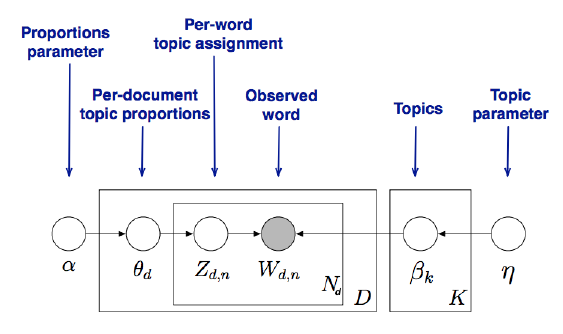
\includegraphics[width=0.7 \textwidth]{Images/platenotation2.png}
\begin{itemize}\setlength{\itemsep}{1em}
\item For each document $d$:
\vspace{4pt}
\begin{itemize}\setlength{\itemsep}{0.8em}
\item Draw topic proportions $\theta_d$ from Dirichlet distribution with parameter $\alpha$ 
\item For each word $n$:
\vspace{4pt}
\begin{itemize}
\setlength{\itemsep}{0.5em}
            \item Draw a topic assignment $Z_{d,n} \sim Multinomial (\theta_d)$
            \item Draw word $W_{d,n} \sim Multinomial (\beta_k)$
        \end{itemize}
    \end{itemize}
\end{itemize}
\end{frame}
%%%%%%%%%%%%%
\begin{frame}{Model: LDA}
\begin{center}
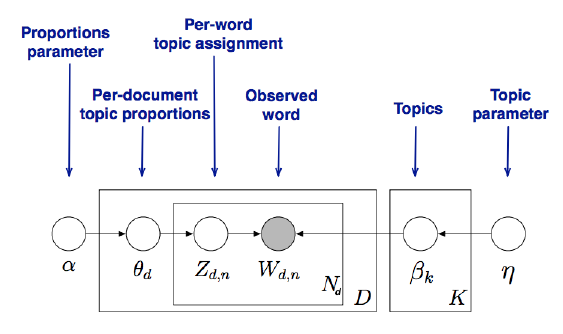
\includegraphics[scale=0.4]{Images/platenotation2.png}
\end{center}
\begin{itemize}
\item \textcolor{blue}{$\alpha$:} document-topic density
\begin{itemize}
    \item higher $\alpha$ means documents contain more topics, lower $\alpha$ means documents contain fewer topics
\end{itemize}
\item \textcolor{blue}{$\eta$:} topic-word density
\begin{itemize}
    \item higher $\eta$ means topics have more words, lower $\eta$ means topics have fewer words
\end{itemize}
\item For each word in $N_d$ plate, we have a variable $Z_{d,n}$ which gives the topic assignment for the $n$-th word drawn from the $\theta_d$ distribution
\end{itemize}
\end{frame}
%%%%%%%%%%%%%%
\begin{frame}{Model: Dirichlet distribution}
\begin{itemize}
\setlength{\itemsep}{1.5em}
    \item The Dirichlet distribution is an exponential family distribution over the simplex of positive numbers that sum to one
    \begin{itemize}\vspace{5pt}
        \item It is a pdf over the set of all multinomial parameter vectors
    \end{itemize}
    \item The Dirichlet distribution is a \textcolor{blue}{distribution over distributions}
$$
p(\mathbf{p} \mid \alpha)=\frac{\Gamma\left(\sum_{i=1}^{k} \alpha_{i}\right)}{\prod_{i=1}^{k} \Gamma\left(\alpha_{i}\right)} \prod_{i=1}^{k} p_{i}^{\alpha_{i}-1}
$$
where $\sum p_{i}=1$ and $p_{i} \geq 0$
\item \textcolor{blue}{Key property:} As $\alpha$ gets smaller, the distribution becomes more sparse
\begin{itemize}\vspace{5pt}
    \item sparsity is a feature of text data
\end{itemize}
\end{itemize}
\end{frame}
%%%%%%%%%%%%%%
\begin{frame}{The case of $k=3$}
\begin{center}
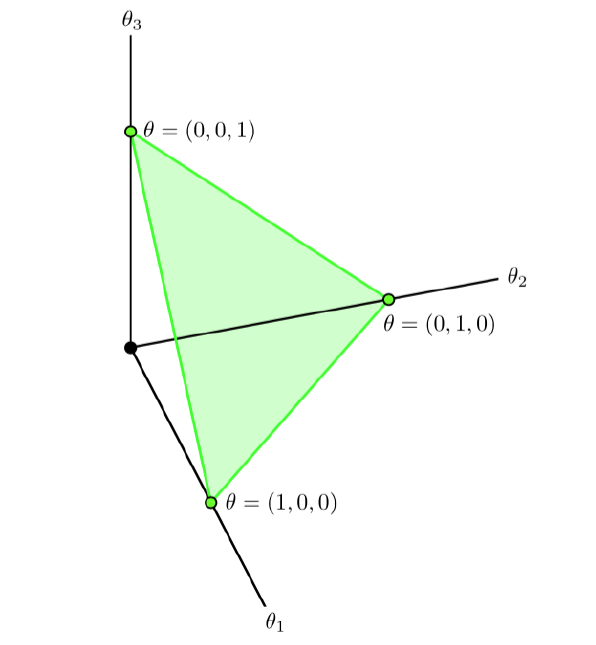
\includegraphics[scale=0.37]{Images/case3.png}
\end{center}
\end{frame}
%%%%%%%%%%%%%%
\begin{frame}{The case of $k=3$ and $\alpha_j = 1$}
\begin{center}
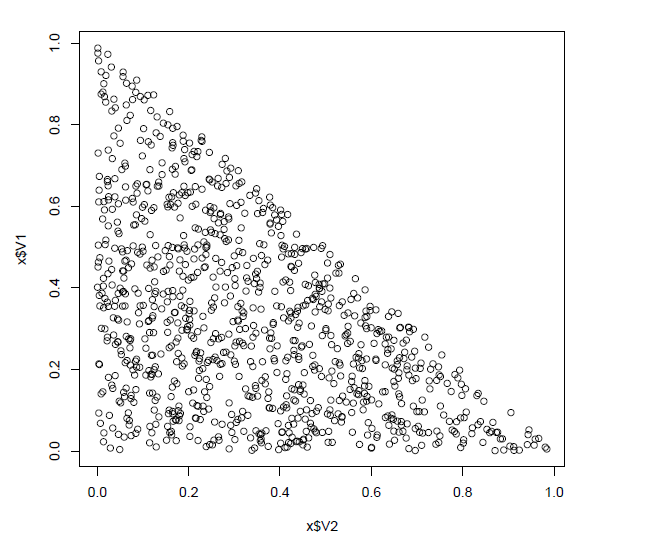
\includegraphics[scale=0.45]{Images/case3a.png}
\end{center}
\end{frame}
%%%%%%%%%%%%%%
\begin{frame}{The case of $k=3$ and $\alpha_j = 10$}
\begin{center}
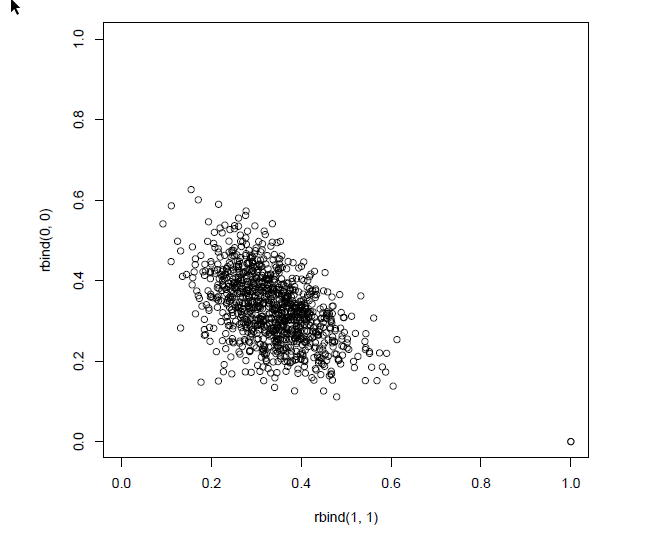
\includegraphics[scale=0.45]{Images/case3b.png}
\end{center}
\end{frame}
%%%%%%%%%%%%%%
\begin{frame}{The case of $k=3$ and $\alpha_j = 0.25$}
\begin{center}
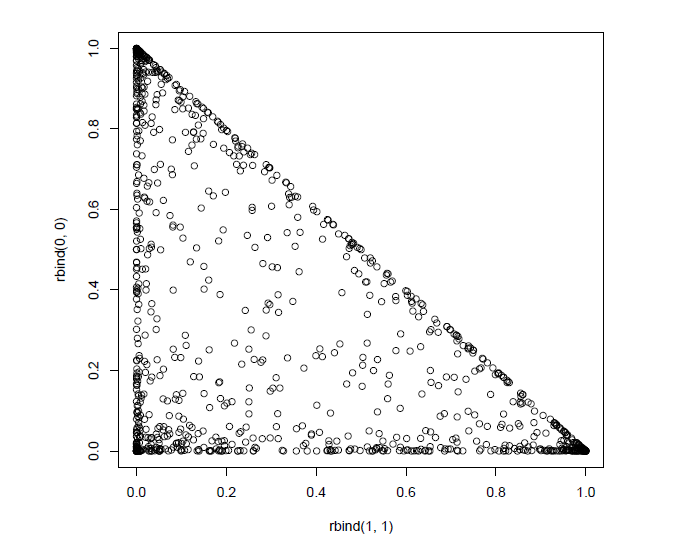
\includegraphics[scale=0.45]{Images/case3c.png}
\end{center}
\end{frame}
%%%%%%%%%%%%%%
\begin{frame}{The case of $k=3$ and $\alpha_j = 0.05$}
\begin{center}
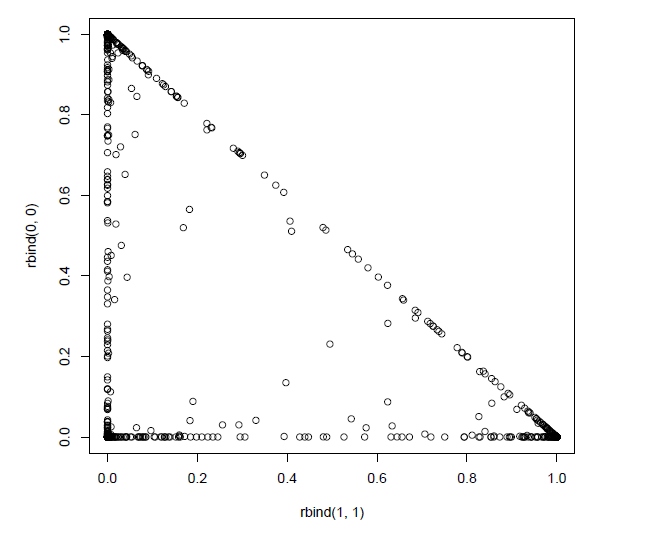
\includegraphics[scale=0.45]{Images/case3d.png}
\end{center}
\end{frame}
%%%%%%%%%%%%%%
\begin{frame}{Model: static LDA}
\begin{itemize}
\setlength{\itemsep}{1.2em}
    \item Where is the information for each word's topic?
    \begin{itemize}\vspace{5pt}
        \item we are learning the pattern of what words occur together
    \end{itemize}
    \item The model wants
    \begin{itemize}\vspace{5pt}\setlength{\itemsep}{0.5em}
        \item a \textcolor{blue}{topic} to contain as few words as possible
        \item but a document to contain as few \textcolor{blue}{topics} as possible
    \end{itemize}
\item This tension is what makes the original LDA model (Blei et al. 2003) work, which is static
\item Data generating process is i.i.d. across words within a document and across all documents that draw on the topic proportions 
\item E.g., same probability of talking about a topic in 1880 and 2000!
\end{itemize}
\end{frame}
%%%%%%%%%%%%%%
\begin{frame}{Model: dynamic LDA}
%\begin{itemize}
%    \item Documents are exchangeable; in many settings of interest, topics evolve systematically over time
%\end{itemize}
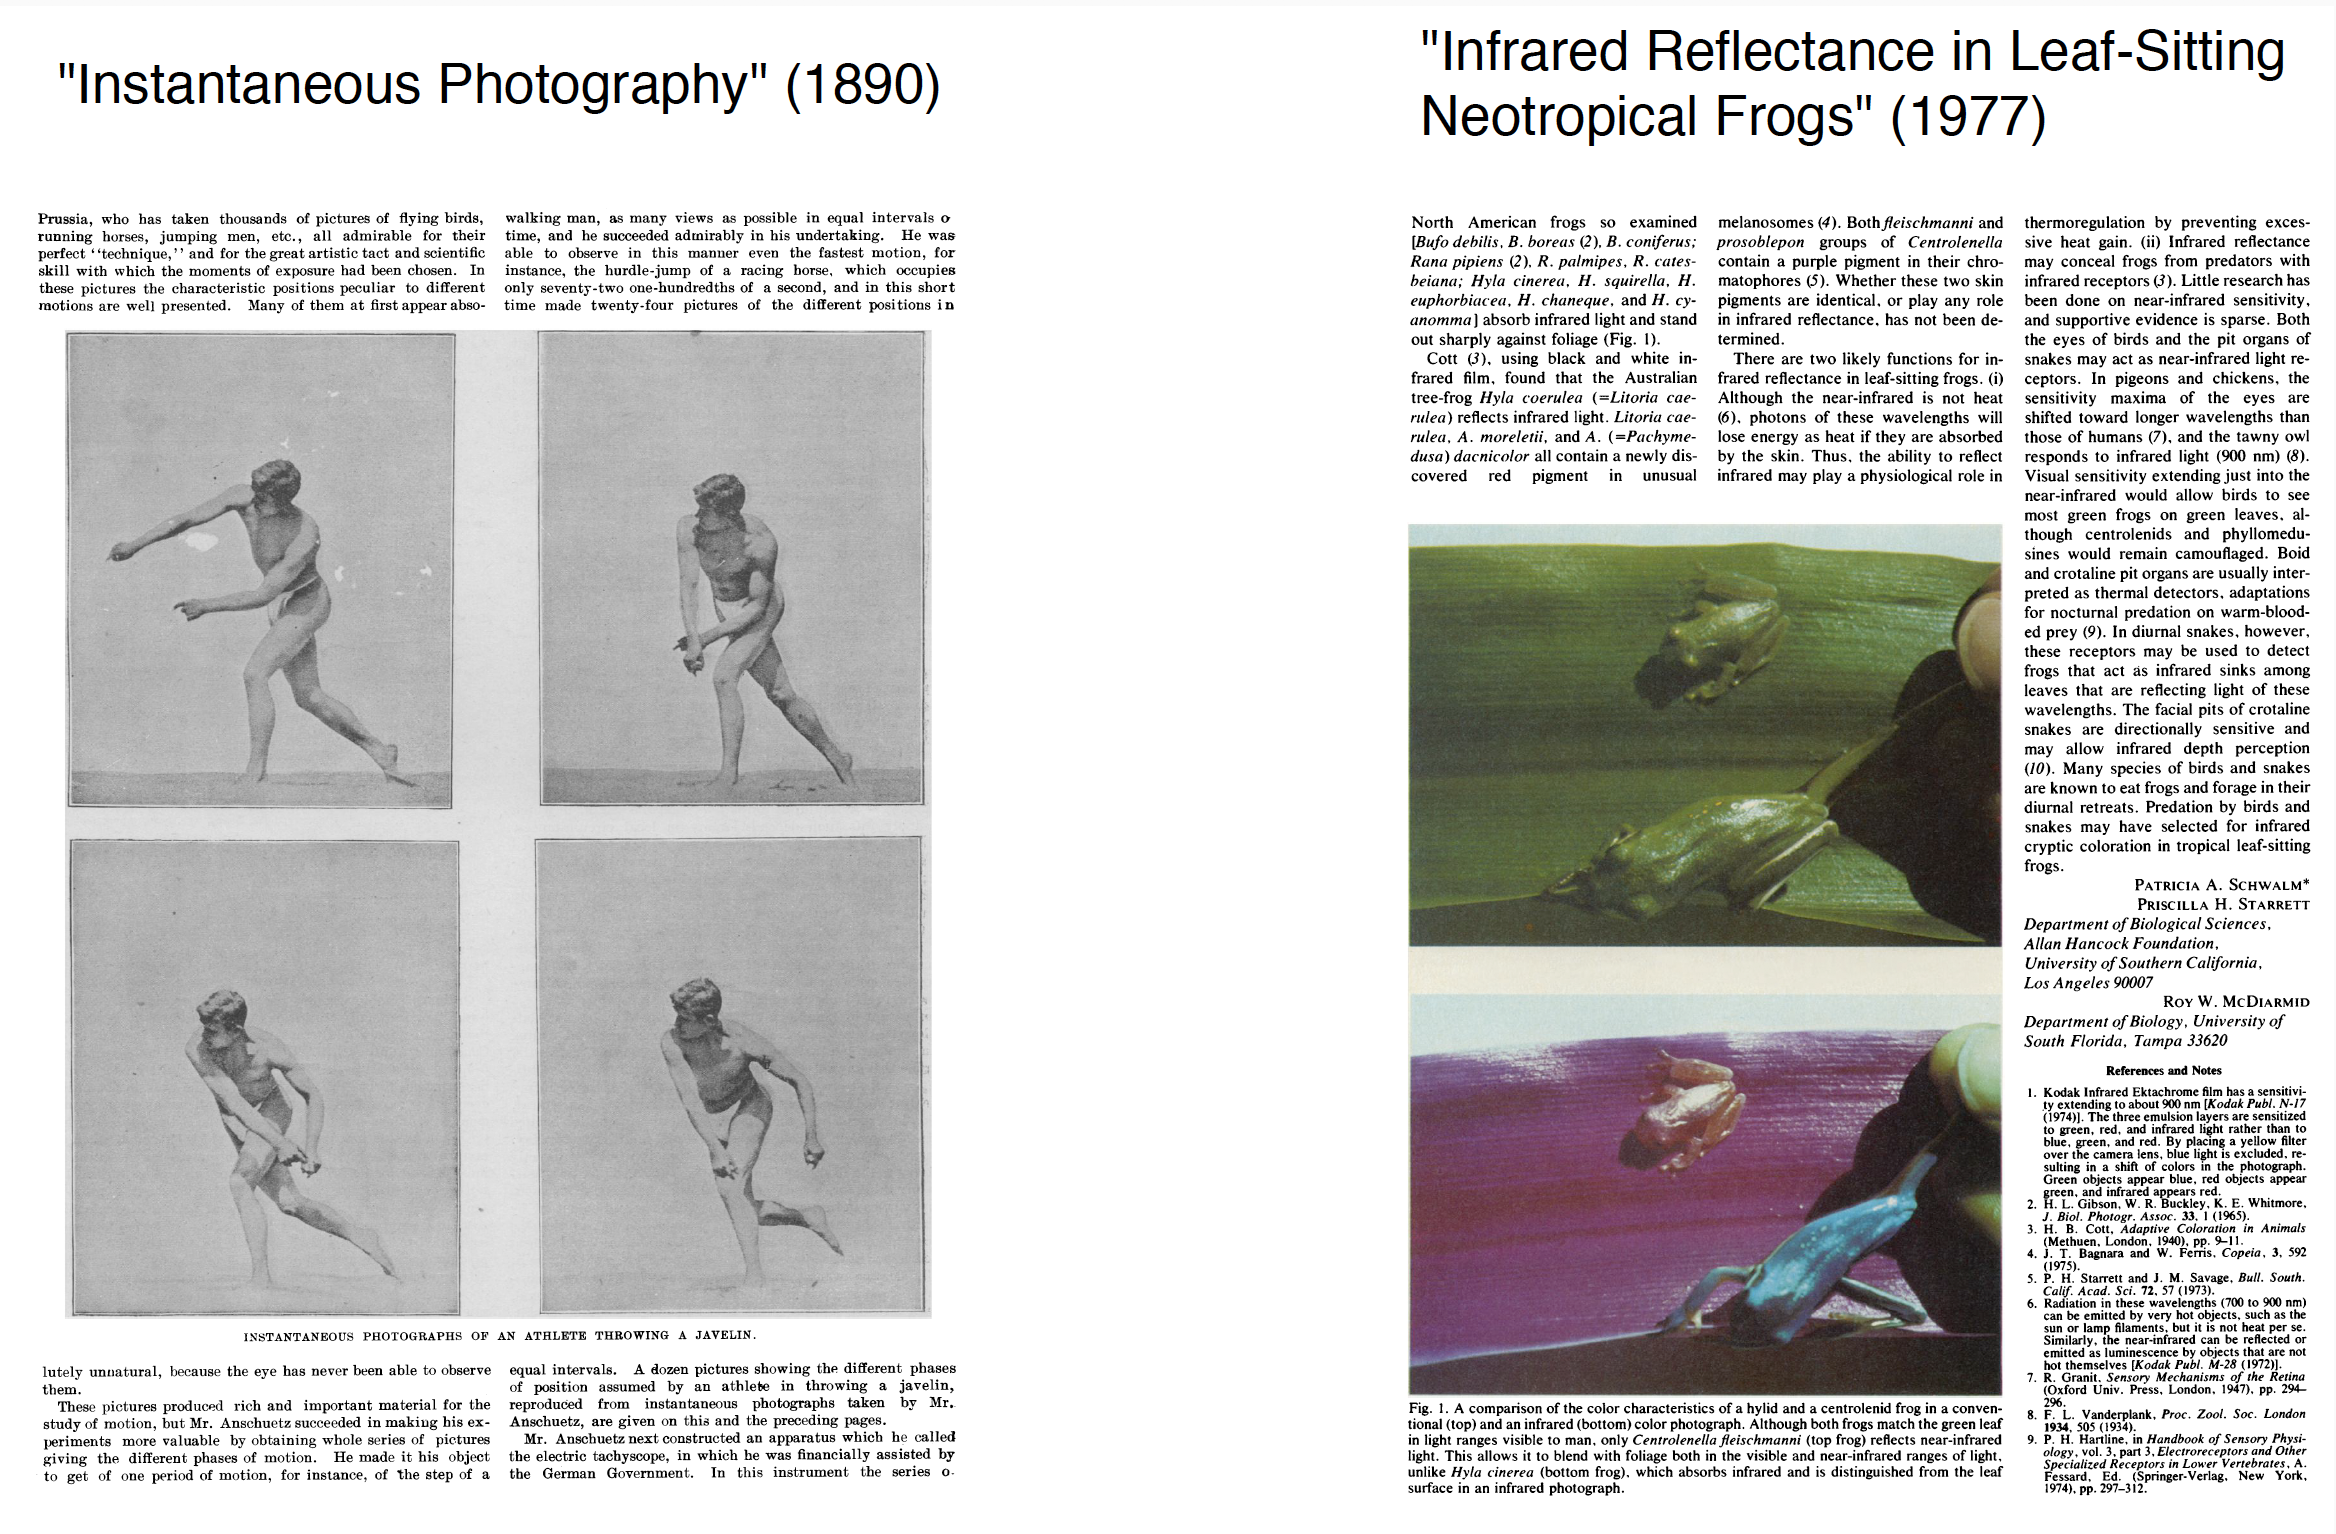
\includegraphics[width=0.9 \textwidth]{Images/photos_overtime.png}
\end{frame}

\begin{frame}{Model: dynamic LDA}
\begin{itemize}
\setlength{\itemsep}{1em}
    \item Divide text into sequential slices (e.g., by year)
    \item Assume each slice's documents drawn from LDA model
    \item Allow word distribution within topics and distribution over topics to change smoothly over time via Markov process
\end{itemize}
\end{frame}

\begin{frame}{Estimation}
\begin{itemize}
\setlength{\itemsep}{1em}
    \item Bayesian inference intractable using standard methods (e.g. Gibbs sampling)
    \vspace{6pt}
    \begin{itemize}
    \setlength{\itemsep}{0.6em}
        \item Blei (2006) $\rightarrow$ variational inference
        \item Taddy R package $\rightarrow$ MAP estimation
        \item Current favorite $\rightarrow$ Stochastic gradient descent
    \end{itemize}
    \item Main estimate if for 20 topic models
\end{itemize}
    
\end{frame}

\begin{frame}{Results: dynamic LDA}
\begin{center}
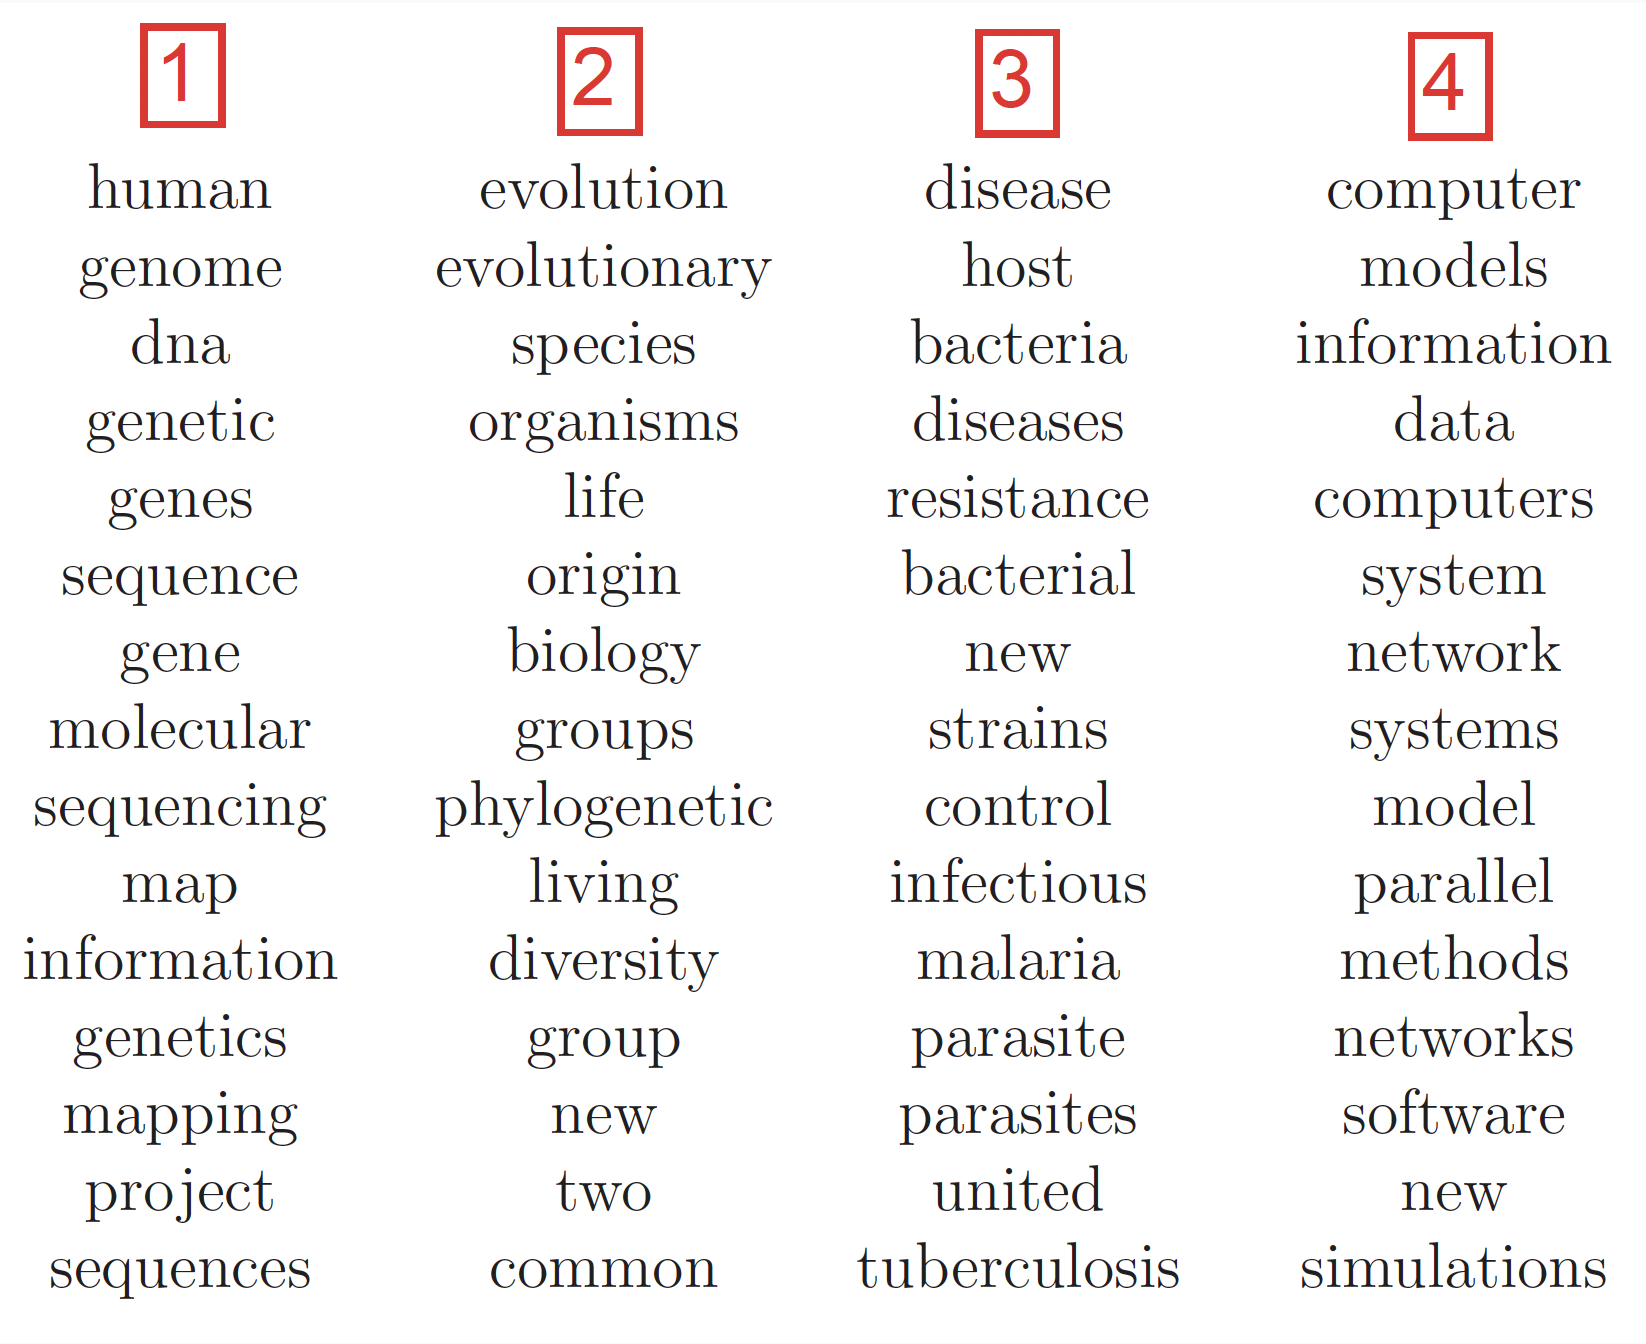
\includegraphics[width=0.9 \textwidth]{Images/topics_output.png}
\end{center}
\end{frame}

\begin{frame}{Results: dynamic LDA}
\centering
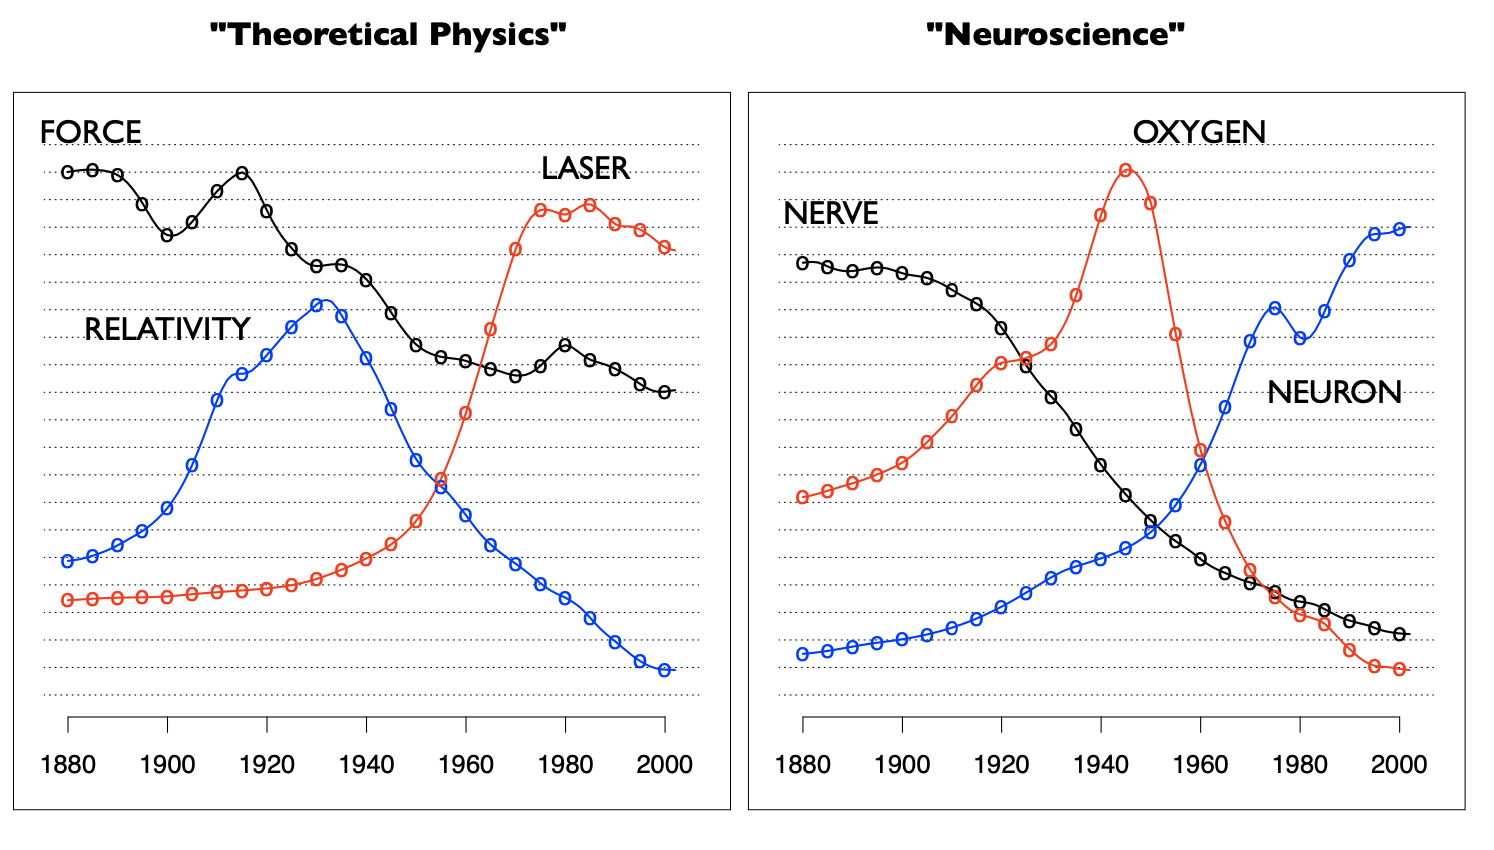
\includegraphics[width=1 \textwidth]{Images/dynamic_trends.png} 

\begin{itemize}
\setlength{\itemsep}{0.6em}
\item These are the $\beta$ loadings on these words in a given topic over time 
\end{itemize}
\end{frame}

\begin{frame}{Results: dynamic LDA}
\centering
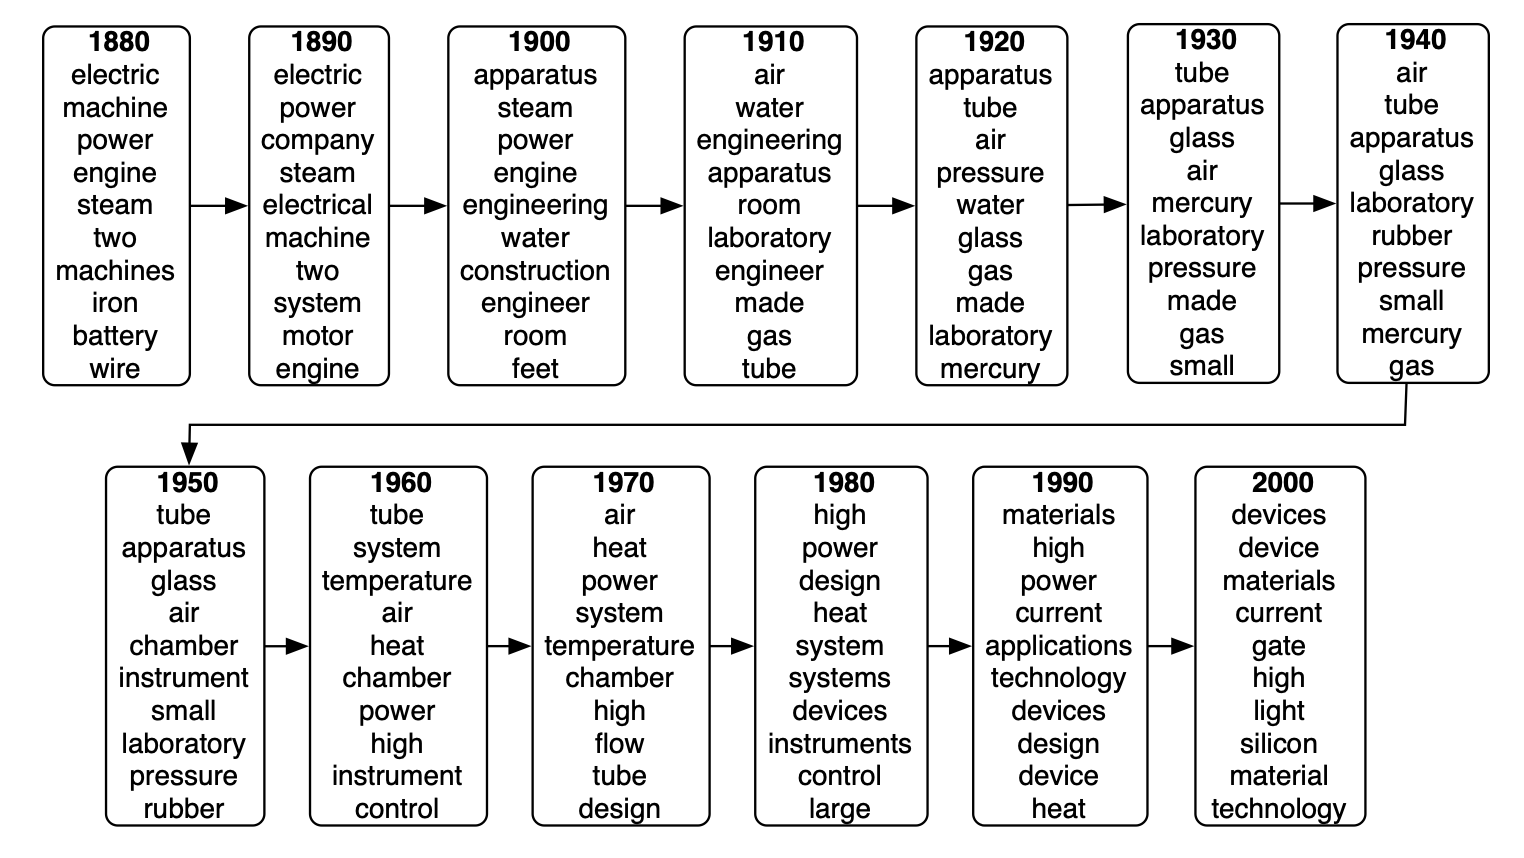
\includegraphics[width=1 \textwidth]{Images/dynamic_results.png} 
\end{frame}

\begin{frame}{Results: dynamic LDA}
\centering
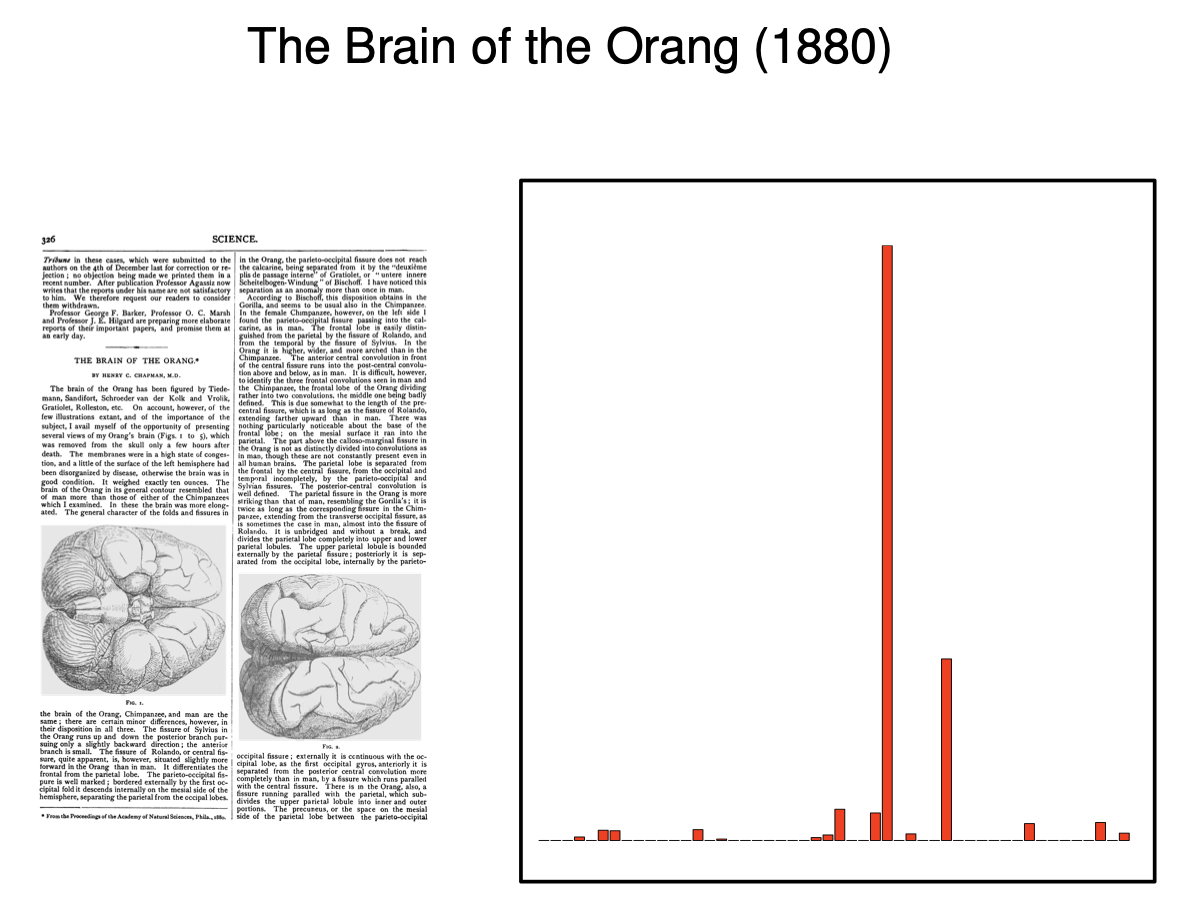
\includegraphics[width=0.9 \textwidth]{Images/brain_orang.png} 
\end{frame}

\begin{frame}{Results: dynamic LDA}
\centering
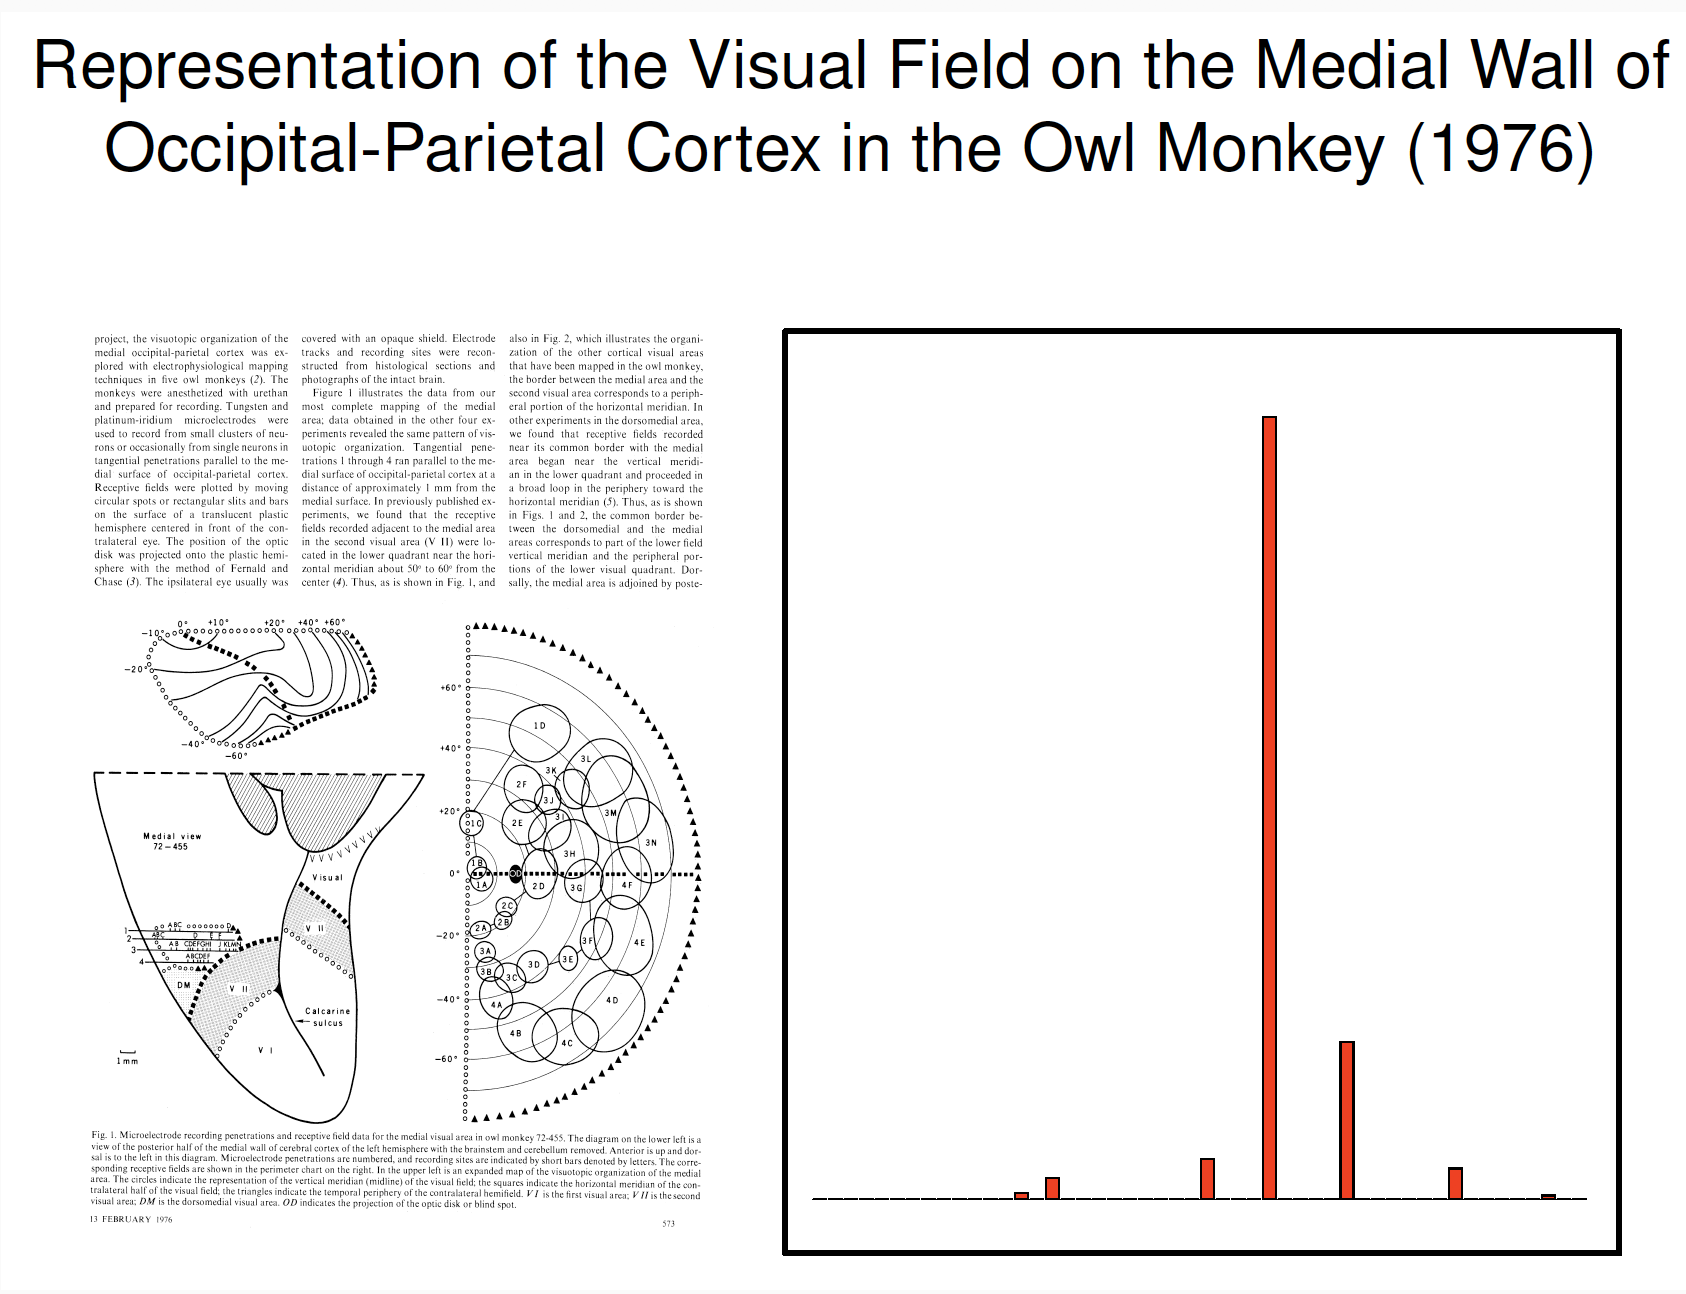
\includegraphics[width=0.9 \textwidth]{Images/brain_orang2.png} 
\end{frame}

\begin{frame}{Quinn et al., 2010: what do U.S. congressmen talk about?}
\centering
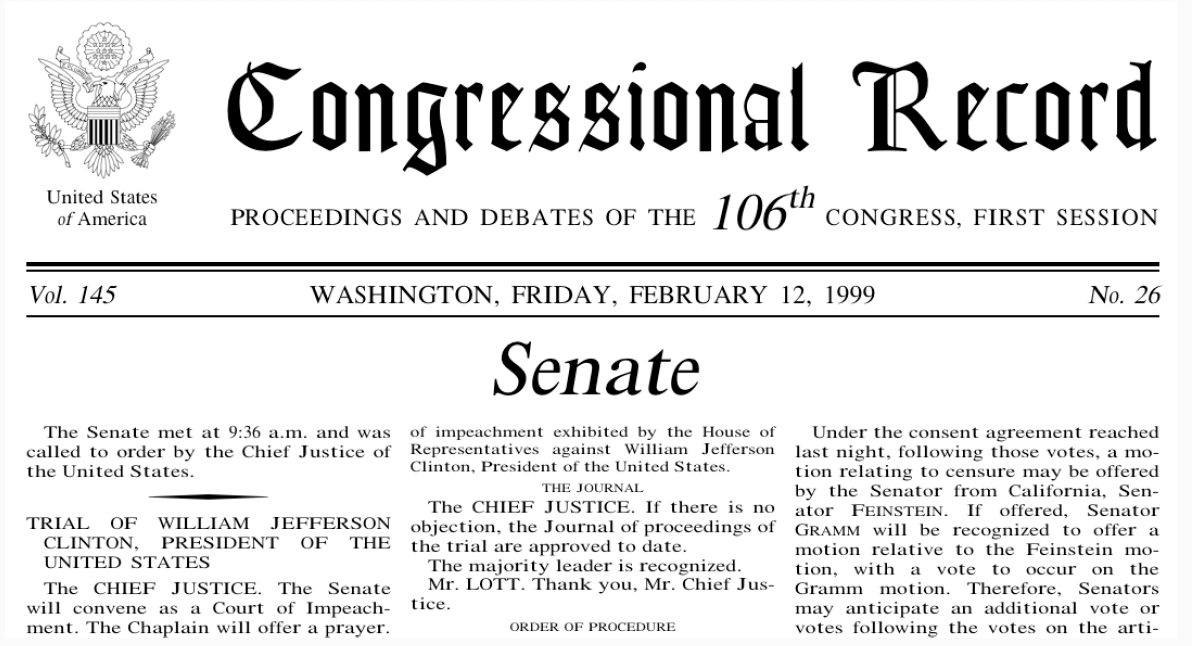
\includegraphics[width=0.8 \textwidth]{Images/congress_records.png} 
\vspace{10pt}
\begin{itemize}
    \item Full text of speeches in US Senate 1995-2004
    \vspace{4pt}
    \begin{itemize}
    \setlength{\itemsep}{0.4em}
     \setlength{\itemindent}{-0.75em}
        \item Count words appearing in 0.5\% or more of speeches (after stemming)
        \item Vocabulary: 3,807 words
        \item Total documents: 118,065 speeches
    \end{itemize}
\end{itemize}
\end{frame}

\begin{frame}{Model}
\begin{itemize}
    \setlength{\itemsep}{1.1em}
    \item Like Blei \& Lafferty (2006) except:
    \vspace{5pt}
    \begin{itemize}
        \setlength{\itemsep}{0.4em}
        \item Each document is in exactly one topic
        \item Dynamic distribution of topics, but topics themselves are static
    \end{itemize}
    \item Blei \& Lafferty: 
    \vspace{5pt}
    \begin{itemize}
        \setlength{\itemsep}{0.4em}
        \item $\textbf{x}_i \sim Multinomial (\beta_1 \theta_{i1} + ... + \beta_k \theta_{ik})$
        \item $\theta_i \sim F (\alpha)$
        \item $\beta$ and $\alpha$ both evolve over time
    \end{itemize}
    \item Quinn et al. (2010):
    \vspace{5pt}
    \begin{itemize}
        \setlength{\itemsep}{0.4em}
        \item $\textbf{x}_i \sim Multinomial (\beta_{k(i)})$
        \item $Pr(k(i) = j) = \alpha_j$
        \item $\alpha$ evolves over time; $\beta$ constant
    \end{itemize}
\end{itemize}
\end{frame}

\begin{frame}{Estimation}
\begin{itemize}
        \setlength{\itemsep}{0.8em}
    \item Estimate using maximum likelihood using ECM algorithm
    \item Main estimates are for 42 topic models (chosen based on ``substantive and conceptual'' criteria)
\end{itemize}
\end{frame}

\begin{frame}{Estimation}
\centering
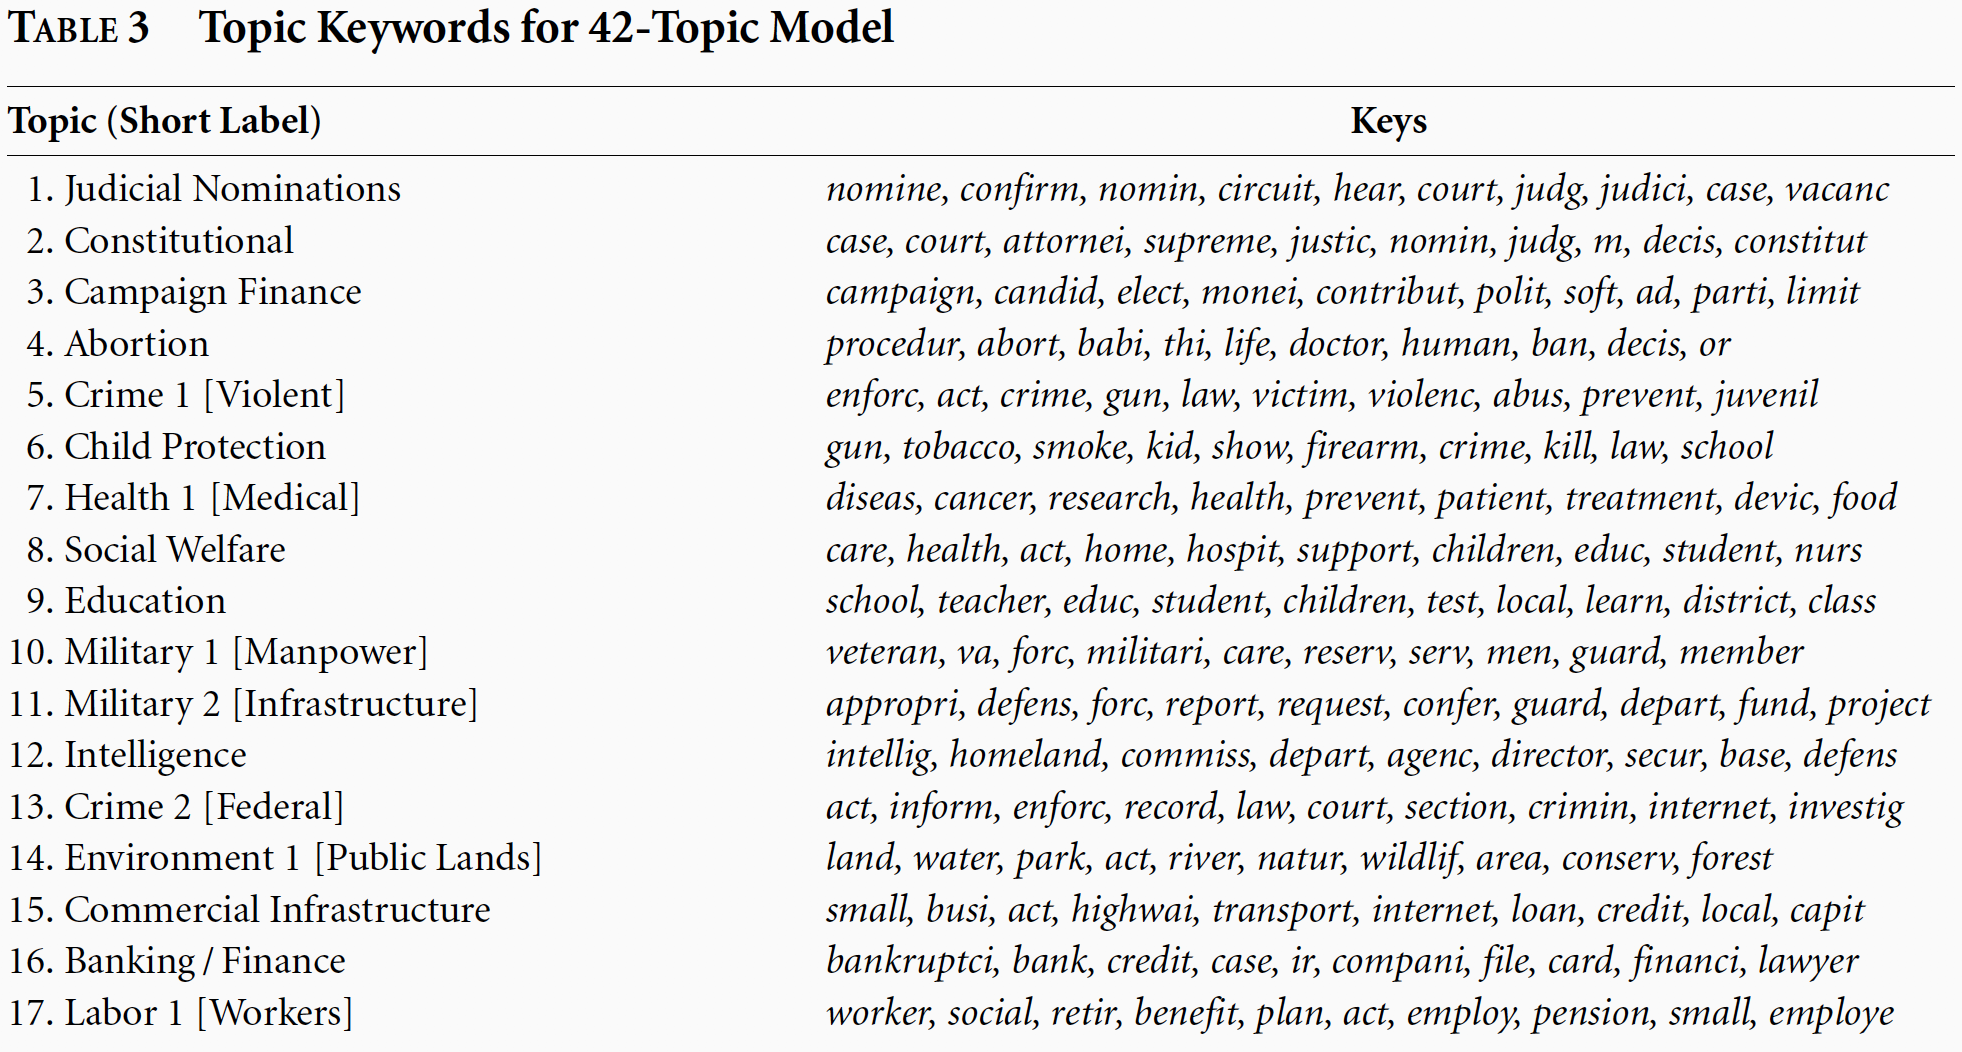
\includegraphics[width=1 \textwidth]{Images/table_quinn.png}
\end{frame}


\begin{frame}{}
    \centering
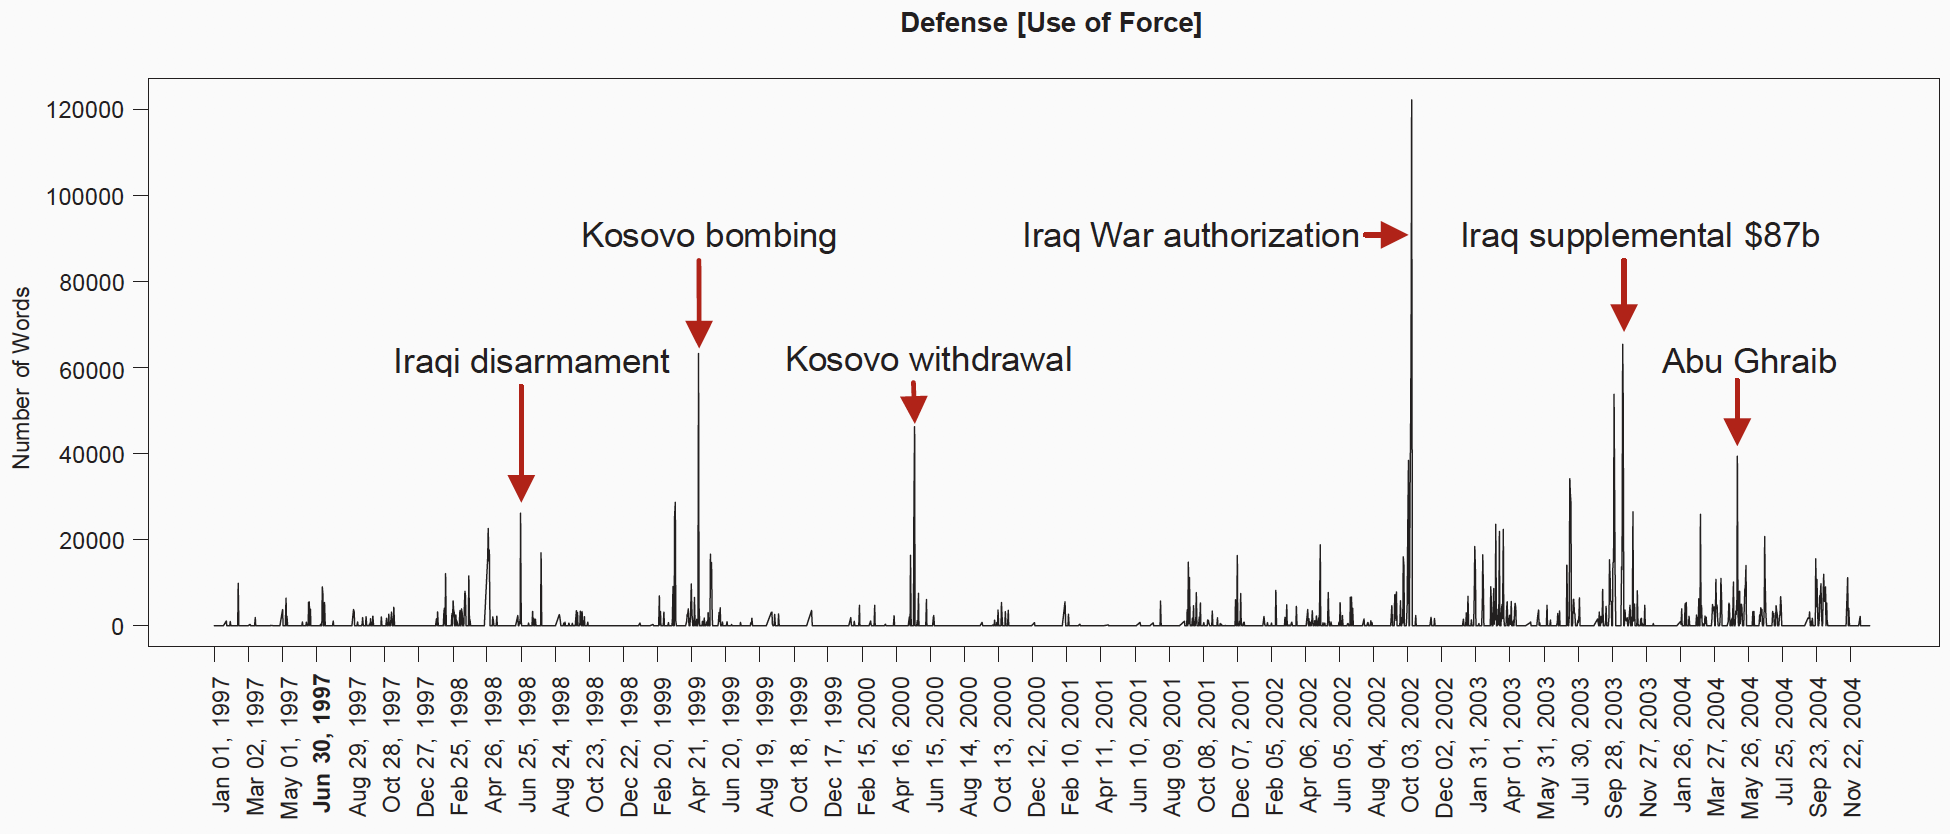
\includegraphics[width=1 \textwidth]{Images/use_force.png}
\end{frame}

\begin{frame}{}
    \centering
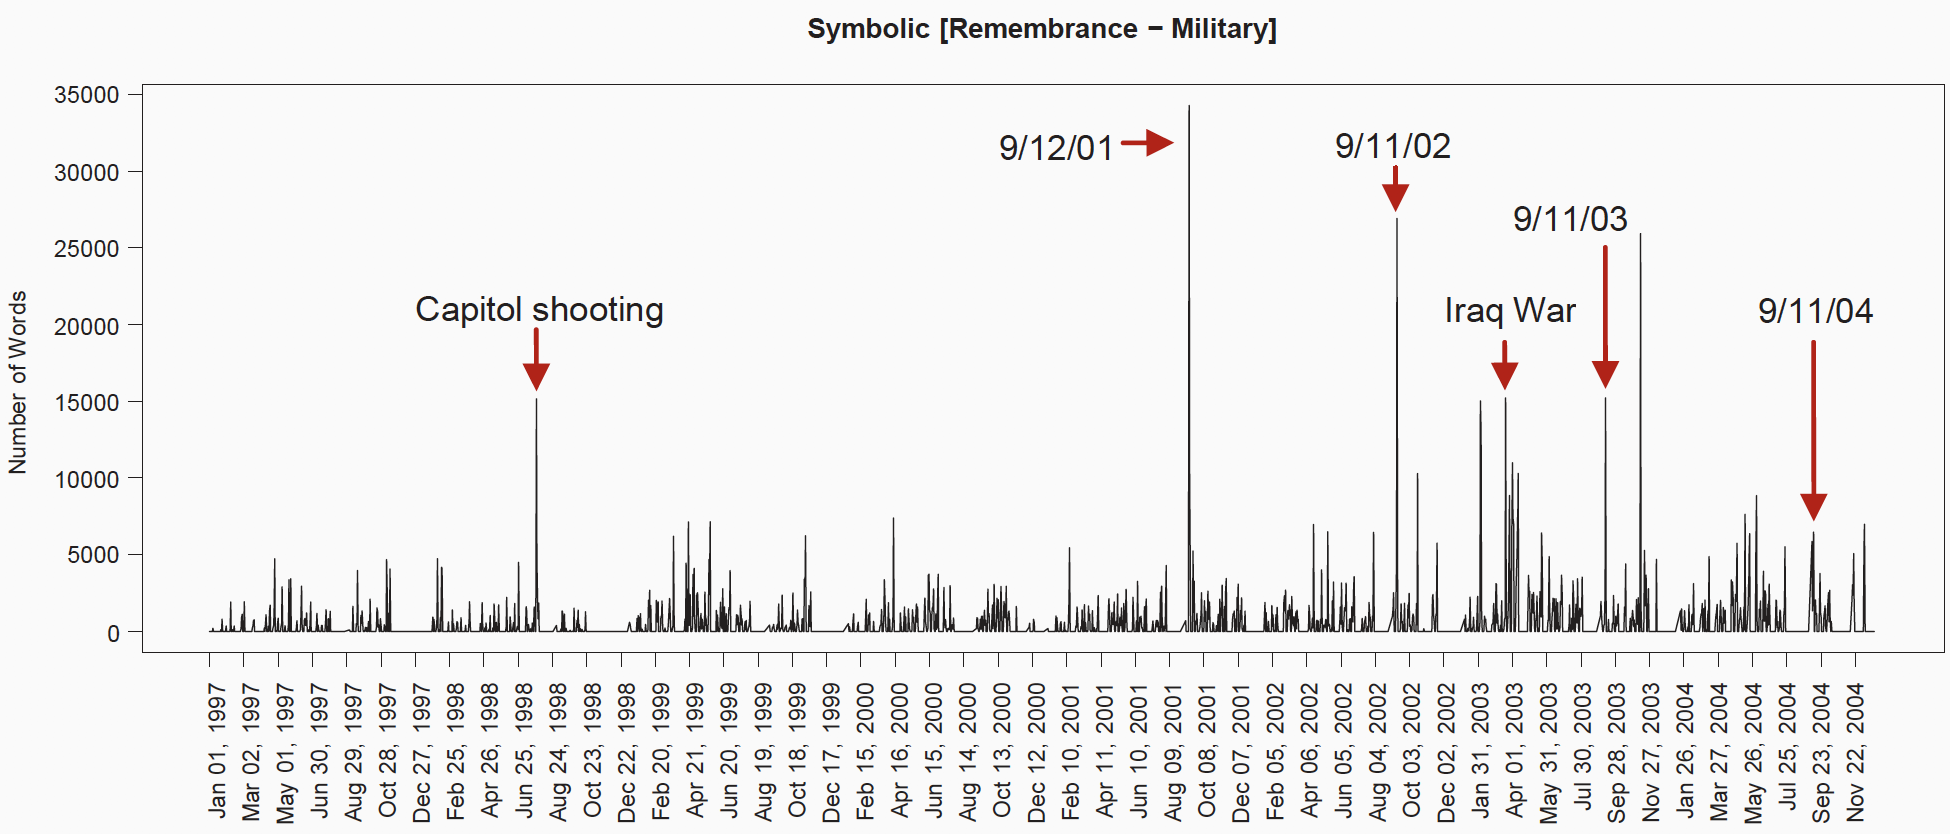
\includegraphics[width=1 \textwidth]{Images/military.png}
\end{frame}

% This doesn't make much sense imo
\begin{frame}{}
    \centering
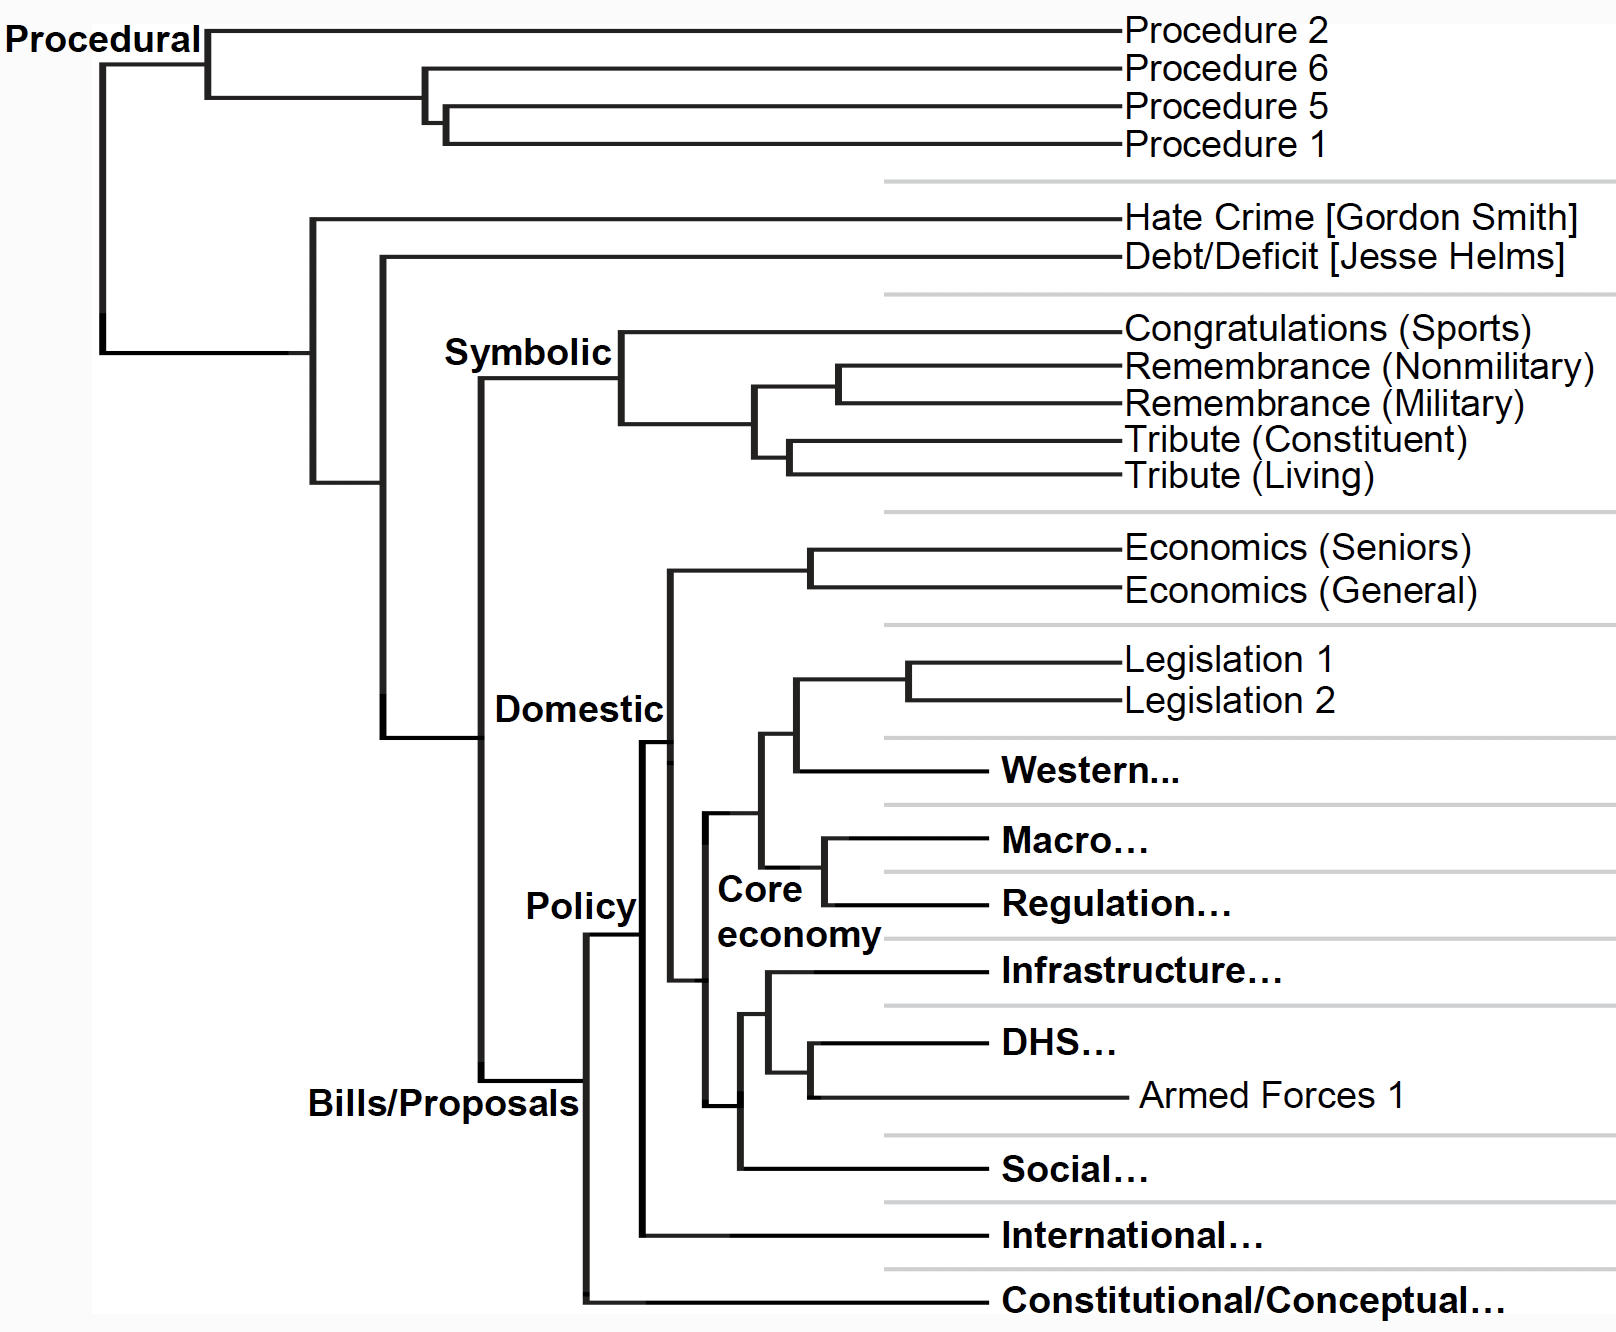
\includegraphics[width=0.8 \textwidth]{Images/procedures.png}
\end{frame}


\begin{frame}{Hansen, McMahon and Prat (2018): FOMC transparency}
\begin{itemize}
\setlength{\itemsep}{1.5em}
\item Goal: analyze how making the Federal Reserve monetary policy meetings more \textcolor{blue}{transparent} affect the policymakers' incentives and their discussion
\item Motivation: enhanced transparency
\begin{itemize}
    \item Can incentivize effort and relevant contributions, a \textcolor{blue}{discipline} effect
% That is, increases accountability, induces them to work harder and behave better.
    \item Can discourage broad and creative debate, a \textcolor{red}{conformity} effect
% They may engage in either herding and conformism (specially considering this is Greenspan's era) or antiherdism and anticonformism. The results confirm the former.
\end{itemize}
\item Idea: use changes in the Federal Reserve's disclosure policy and transcripts in years both before and after the change to exploit variation in communication patterns
% The authors use LDA with topics K = 40 on a corpus of 26,645 statements with 24,314 unique words. LDA generates probabilities of words in statements being categorized in a topic, and these conditional distributions over policy topics are then used to measure differences and diversity in topics discussed per member, their focus on quantitative vs. qualitative data, and their number of statements. These "Communication measures" are then regressed as a Diff-in-Diff and show how members' realization that their statements were public conditioned their response behavior. 

\item \textcolor{blue}{Main finding:} inexperienced members show increased discipline and focus on quantitative subjects after change. Although they also exhibit a bias toward conformity, the former effect dominates
% Less experienced members discuss a relatively more diverse set of topics after transparency. Instead of focusing on what their colleagues do, they tend to bring new dimensions of policy into their discussions
\end{itemize}
\end{frame}%



\begin{frame}{Hansen, McMahon and Prat (2018): natural experiment}
\begin{itemize}
\setlength{\itemsep}{1.5em}
\item The FOMC meets eight times a year to draft monetary policy and lay out other Federal Reserve policies
\item Authors exploit as a \textcolor{blue}{natural experiment} a change in the Fed's FOMC meetings disclosure policy
\vspace{4pt}
\begin{itemize}
\setlength{\itemsep}{0.4em}
\item \textcolor{blue}{1970-1993:} members thought that their debates were not recorded. Only later did Greenspan discover that meetings had been transcribed

    \item \textcolor{blue}{1993}: after revelation, the Fed agrees to publish all past transcripts and to release any transcripts henceforth with a five-year lag 
% Each policymaker then essentially took for granted that every spoken word would be public after five years

\end{itemize}
\item Difference-in-difference model
\begin{itemize}
    \item Compare experts of varying experience before and after 1993
% Plenty of robustness controls here. The main specification uses members who were present in the FOMC meeting in October 1993. This is intended to work around issues of simultaneous structural changes in the FOMC, the result of Clinton nominating during those years mostly members with academic profiles which may capture some of the treatment effect. 
    \item Idea: rookie FOMC members react stronger due to \textcolor{blue}{career concerns}
% Veteran members without career concerns will spend less time preparing for meetings or paying attention to colleagues during them. Rookie members gather additional data between meetings (more technical wording in statements) and try to bring new dimensions of policy into their discussions (their similarity measures are lower; for measures of these see Table VI).
\end{itemize}
\end{itemize}
\end{frame}%


\begin{frame}{Hansen, McMahon and Prat (2018): empirical strategy}
\begin{itemize}
\setlength{\itemsep}{1.5em}
\item \textcolor{blue}{Documents:} 26,645 recorded member statements with 24,314 unique words
\item \textcolor{blue}{Pre-processing:} collocations, stop-words, stemming, tf-idf weighting. $V=8,206$ unique terms
\item \textcolor{blue}{LDA application}
\vspace{4pt}
\begin{itemize}
\setlength{\itemsep}{0.4em}
    \item Set \textcolor{blue}{K = 40} topics, each a probability vector \textcolor{blue}{$\beta^k$} over all words. 
    % Bandiera uses K=2 in order to maximize interpretability. Hansen uses K=40 in order to increase goodness of fit, although the number is discretionary. Robustness checks with different K are performed.
    \item A document \textcolor{blue}{$d$} has its own distribution over topics given by \textcolor{blue}{$\theta_d$}. \begin{itemize}
        \item Informally, \textcolor{blue}{$\theta^k_d$} represents the share of topic \textcolor{blue}{$k$} in document \textcolor{blue}{$d$}x
    \end{itemize}
    \item Use Dirichlet priors on \textcolor{blue}{$\beta^k$} and \textcolor{blue}{$\theta_d$} and estimate their posterior distributions with Gibbs sampling (Griffiths and Steyvers, 2004)
\end{itemize}
\end{itemize}
\end{frame}%

\begin{frame}{\small{Hansen, McMahon and Prat (2018): topics}}
\vspace{-7pt}
\begin{center}
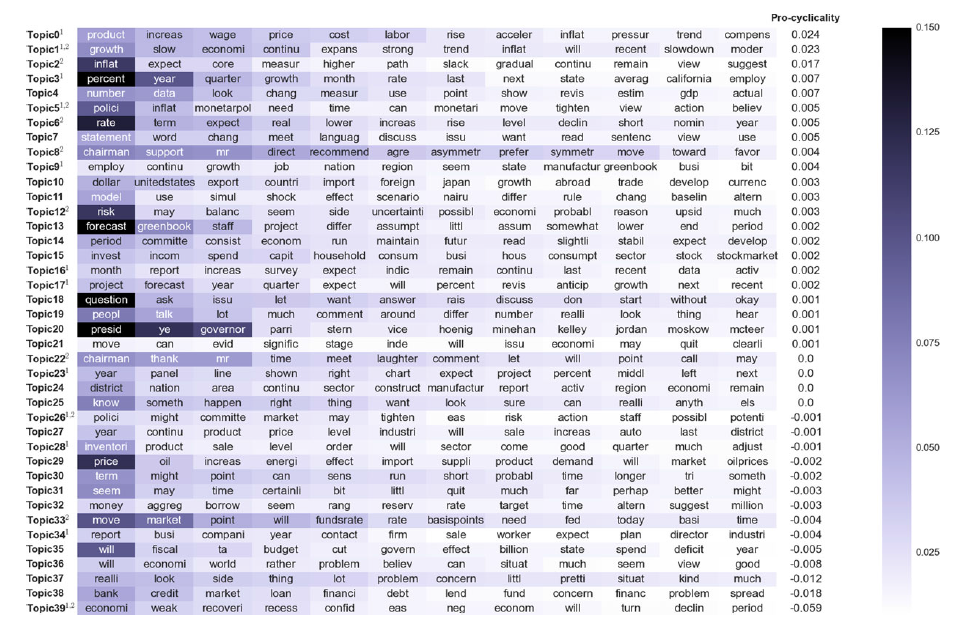
\includegraphics[scale=0.4]{Images/hansen2018a.png}
% This figure summarizes the 40 separate distributions over vocabulary terms that LDA estimates to represent topics. We order these distributions from 0 to 39 based on a procyclicality index that computes the difference in average time the FOMC as a whole spends discussing the corresponding topic in expansions versus contractions, where we use the standard NBER definition of recessions. Within each row, terms are ordered left to right by the probability they appear in each topic, with differential shading indicating approximate probability values.
\end{center}
\end{frame}

\begin{frame}{\small{Hansen, McMahon and Prat (2018): topics}}
\vspace{-7pt}
\begin{center}
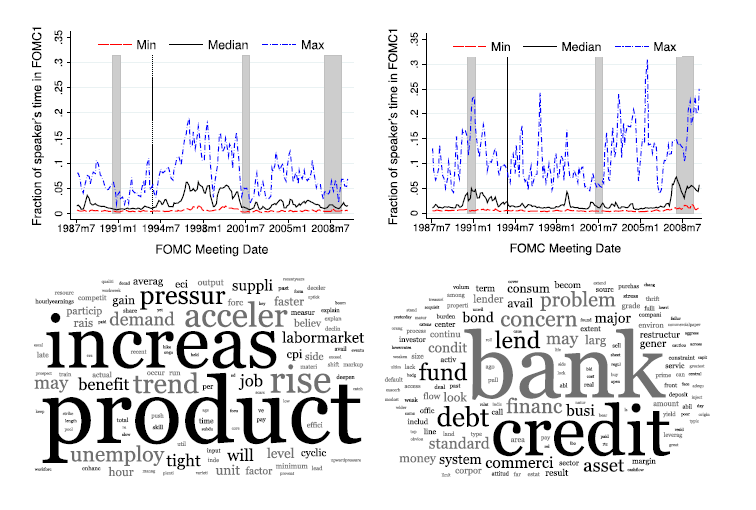
\includegraphics[scale=0.5]{Images/hansen2018b.png}
% This figure shows a topic highly procyclical and a topic highly counter-cyclical
\scalebox{0.8}{
Left panel reflects the most \textcolor{blue}{pro-cyclical} topic; right panel the most \textcolor{blue}{counter-cyclical}
}
\end{center}
\end{frame}

\begin{frame}{\small{Hansen, McMahon and Prat (2018): measures of communication}}
\vspace{-7pt}
\begin{center}
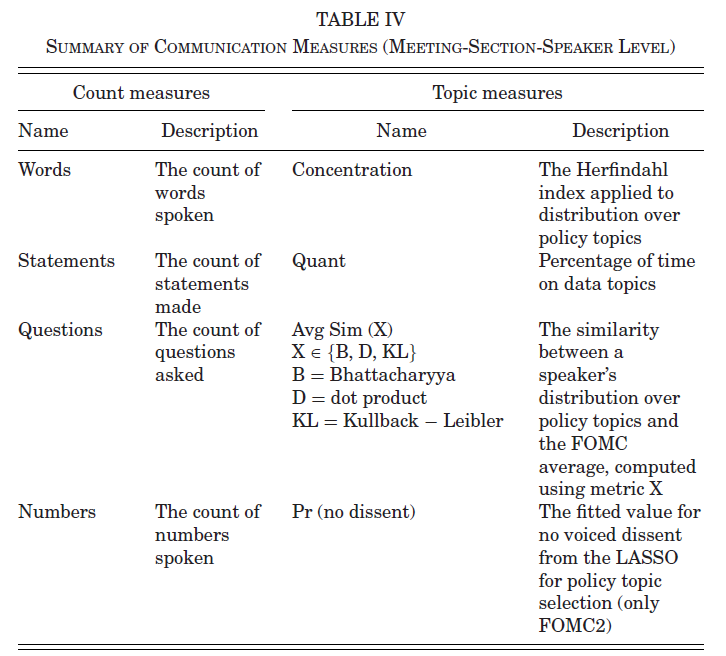
\includegraphics[scale=0.4]{Images/hansen2018c.png}
% This table summarizes empirical measures of communication. These include counts measures on participation and use of numbers and figures by meeting-section(whether economy discussion or policy discussion, FOMC1 & FOMC2 respectively)-member. H-Index measures breadth of deliberation, with high values indicating high concentration and thus a narrow discussion. Measures of similarity use probabilities that speakers may cover a topic and their overlaps. Finally, coefficients from a LASSO are used to map which topics generate the most dissent and are thus more likely to trigger communication differences. 
\end{center}
\end{frame}

% Note on controling for stemms:
%For our topic-based communication measures, we also control for the number of stems that form the topic distributions. This determines the weight the observed data gets in forming the estimated distribution over topics relative to the Dirichlet prior. For example, a member who speaks few stems in a meeting section will have an estimated distribution over topics that is close to uniform, which may induce artificial distance from the committee average.

\begin{frame}{\small{Hansen, McMahon and Prat (2018): results}}
\vspace{-7pt}
\begin{center}
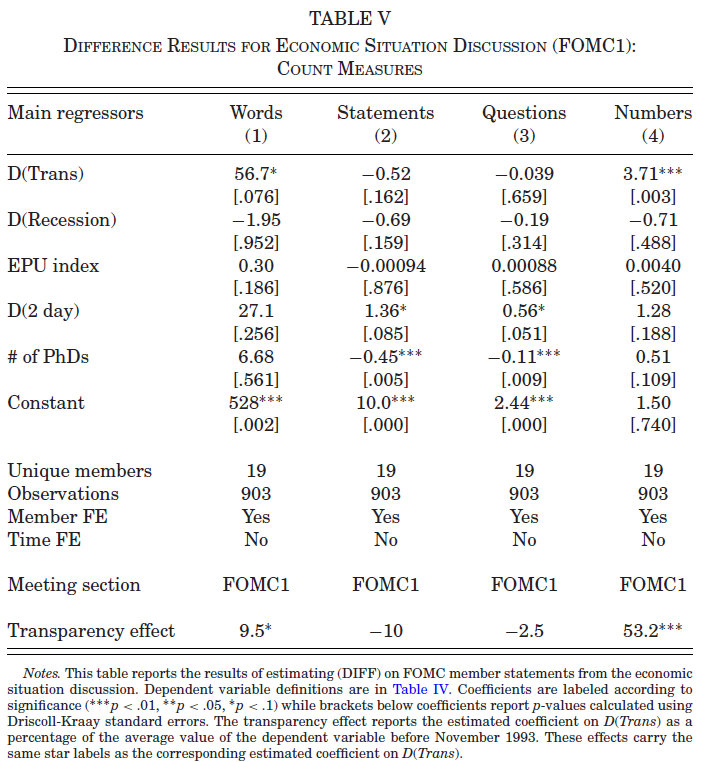
\includegraphics[scale=0.37]{Images/hansen2018d.png}
$$y_{i t}=\alpha_{i}+\gamma D(\text {Trans})_{t}+\lambda X_{t}+\varepsilon_{i t}$$
% Main Diff-in-Diff specification, using as outcome variables the count measures of communication presented above.
\end{center}
\end{frame}

\begin{frame}{\small{Hansen, McMahon and Prat (2018): results}}
\vspace{-7pt}
\begin{center}
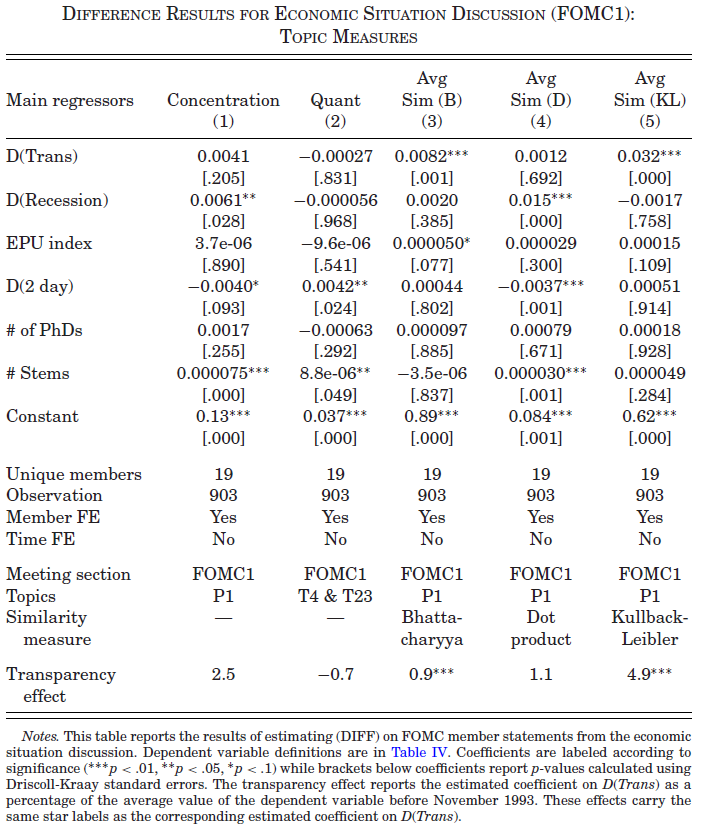
\includegraphics[scale=0.37]{Images/hansen2018e.png}
% Main Diff-in-Diff specification, using as outcome variables the topic measures of communication presented above. A second set of results show the difference in behavior given experience (and thus the rookie argument). These are presented below.
\end{center}
\end{frame}

\begin{frame}{\small{Hansen, McMahon and Prat (2018): results}}
\vspace{-7pt}
\begin{center}
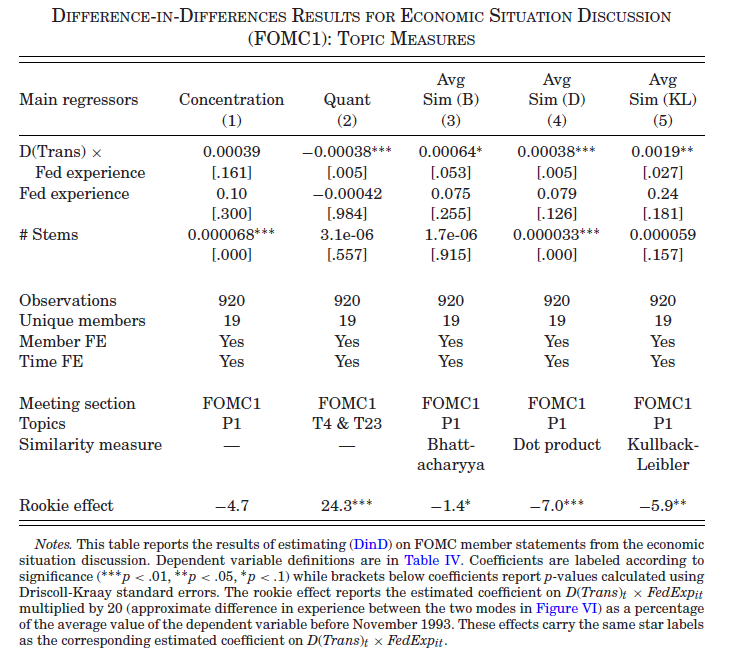
\includegraphics[scale=0.4]{Images/hansen2018f.png}
% A second specification showing the difference in behavior given experience (and thus the rookie argument). The treatment is interacted with the level of fed experience.
\scalebox{0.8}{
Second specification explores change heterogeneity due to \textcolor{blue}{career concerns}
}
\end{center}
\end{frame}


\begin{frame}{Bandiera et al. (2020): measuring CEO behavior}
\begin{itemize}
\setlength{\itemsep}{1.2em}
\item Goal: estimate differences in CEO behavior using high-frequency, high-dimensional diary data and measure their effects on firm performance
\item Idea: generate a one-dimensional behavior index that represents each CEO as a combination of underlying behavioral features 
\item Merge the CEO behavior index with firm balance-sheet data to study the correlation between CEO traits and performance
\item Use a matching model with frictions to alleviate causality reversal concerns and to provide a rationale to firms' observed productivity differentials 
\item \textcolor{blue}{Main finding:} appropriately matched firms and CEOs enjoy better firm performance

\end{itemize}
\end{frame}%

\begin{frame}{Bandiera et al. (2020): survey data}
\begin{itemize}
\setlength{\itemsep}{1.2em}
\item Time allocation survey data on all activities performed in 15-minute time blocks for one week by 1,114 CEOs. Activity types are classified along five different dimensions 
\begin{enumerate}\vspace{5pt}
\setlength{\itemsep}{0.6em}
    \item type (e.g. meeting, public event, etc.)
    \item duration (15 min, 30 min, etc.)
    \item planning (planned or unplanned)
    \item number of participants (one, more than one)
    \item functions of participants (insiders, outsiders)
\end{enumerate}
\item Data has 43,233 separate activities and 4,253 unique type combinations.  
\item One can summarize the data with a 1,114 x 4,253 matrix where the $(i,j)$th element is the number of 15-minute time blocks that CEO $i$ spends in activities with a particular combination of features $j$.
\end{itemize}
\end{frame}%

\begin{frame}{Bandiera et al. (2020): LDA application}
\begin{itemize}
\setlength{\itemsep}{1.5em}
\item Exploit the idea that the high-dimensional raw activity data is generated by a low-dimensional set of latent managerial behaviors
\item Suppose that managers have \textcolor{blue}{$A$} possible ways of organizing each 15-minute block, with \textcolor{blue}{$x_a$} being a particular activity. 
\item If $X \equiv \{x_1,...x_A\}$ is the set of activities, a \textit{pure behavior \textcolor{blue}{$k$}} is the probability distribution \textcolor{blue}{$\beta^k$} over $X$ that is common to all CEOs
\item Set \textcolor{blue}{$K=2$}, so that only two pure behaviors are possible: \textit{managers} and \textit{leaders}. The behavior of CEO \textcolor{blue}{$i$} is given by a mixture of these two behaviors, according to weights \textcolor{blue}{$\theta_i$} $\in [0,1]$

\item The probability of CEO \textcolor{blue}{$i$} generating activity \textcolor{blue}{$a$} can lie anywhere between \textcolor{blue}{$\beta^k_0$} and \textcolor{blue}{$\beta^k_1$}.

\end{itemize}
\end{frame}%

\begin{frame}{Bandiera et al. (2020): LDA application}
\begin{itemize}
\setlength{\itemsep}{1.5em}
\item For each activity of CEO \textcolor{blue}{$i$}, one of the two pure behaviors is drawn independently, given \textcolor{blue}{$\theta_i$}
\item Given the pure behavior, an activity is drawn according to its distribution (either \textcolor{blue}{$\beta_0$} or \textcolor{blue}{$\beta_1$}). The probability that CEO \textcolor{blue}{$i$} assigns to activity \textcolor{blue}{$x_a$} is then 
$$
\chi_{a}^{i} \equiv\left(1-\theta_{i}\right) \beta_{a}^{0}+\theta_{i} \beta_{a}^{1}
$$
\item Let $n_{i,a}$ be the number of times activity \textcolor{blue}{$a$} appears in the time use of CEO \textcolor{blue}{$i$}, then the likelihood function for the model is $$\prod_{i} \prod_{a} \chi_{i}^{n_{i}}$$
\end{itemize}
\end{frame}%

\begin{frame}{\small{Bandiera et al. (2020): LDA application}}
\vspace{-7pt}
\begin{center}
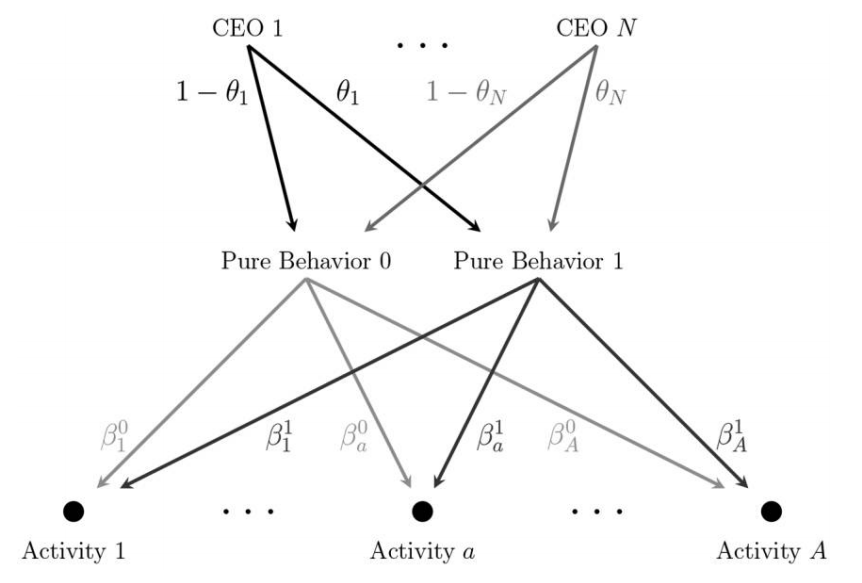
\includegraphics[scale=0.5]{Images/bandiera2017.png}
\end{center}
\end{frame}

\begin{frame}{Bandiera et al. (2020): LDA application}
\begin{itemize}
\setlength{\itemsep}{1.5em}
\item Use Dirichlet priors to \textcolor{blue}{$\beta^k$} and \textcolor{blue}{$\theta_i$}
\item Estimate posterior distributions for \textcolor{blue}{$\beta^k$} and \textcolor{blue}{$\theta_i$} with Gibbs sampling (Griffiths and Steyvers (2004)
\item The process above churns out
\begin{itemize}
    \item two estimated pure behaviors \textcolor{blue}{$\beta^0$} and \textcolor{blue}{$\beta^1$}
    \item the estimated behavior indices \textcolor{blue}{$\hat{\theta}_i$} for CEO \textcolor{blue}{$i$} $= 1,...,N$
\end{itemize}
\end{itemize}
\end{frame}%

\begin{frame}{Bandiera et al. (2020): LDA application}
\vspace{-7pt}
\begin{center}
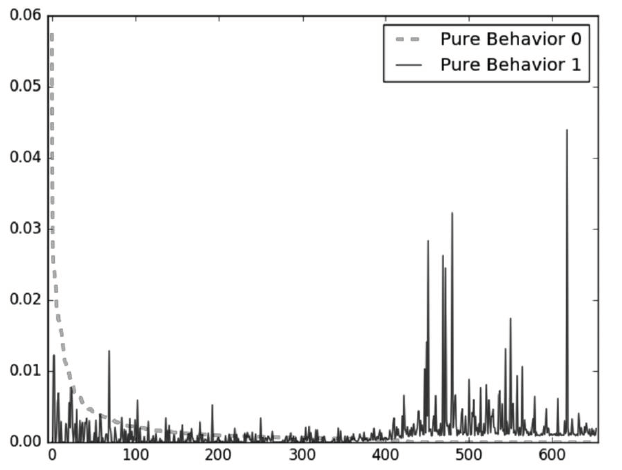
\includegraphics[scale=0.5]{Images/bandiera2017b.png}
\end{center}
\begin{itemize}
    \item Probabilities of activities in estimated pure behaviors. 654 informative activities are ordered in the horizontal axis
\end{itemize}
\end{frame}

\begin{frame}{Bandiera et al. (2020): LDA application}
\vspace{-7pt}
\begin{center}

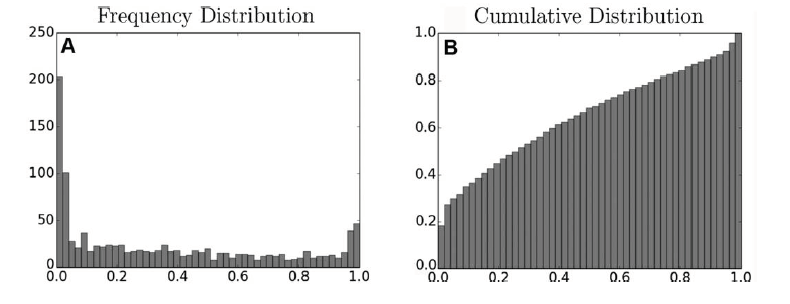
\includegraphics[scale=0.5]{Images/bandiera2017c.png}
\end{center}
\begin{itemize}
    \item Panel A shows number of CEO with behavioral indices in one of 50 bins that divide the space $[0,1]$. Panel B shows the cumulative percentage of CEOs with behavioral indices lying in these bins
\end{itemize}
\end{frame}

\begin{frame}{Barbera et al. (2019): who follows? who leads?}
    \begin{itemize}\setlength{\itemsep}{1.5em}
    \item Who sets the political agenda is an unanswered issue in PoliSci due to data limitations
    \item Apply LDA to social media data (from Twitter) to answer related longstanding questions:
    \begin{itemize}\setlength{\itemsep}{1em}\vspace{5pt}
        \item Are legislators responsive to the priorities of the public?
        \item Which group of voters lead the political agenda?
        \item Do traditional media outlets play any role?
    \end{itemize}
    \item Important consequences on representation and polarization
    \end{itemize}
\end{frame}

\begin{frame}{Barbera et al. (2019): data}
 \begin{itemize}\setlength{\itemsep}{1.2em}
        \item Idea: social media can be used as a source of data on issue salience
        \item Use tweets as a proxy to obtain fine-grain measures of attention being paid to political issues
        \item Collect tweets by a variety of actors during the 113th US Congress (2013-14):
        \begin{itemize}\setlength{\itemsep}{0.6em}\vspace{5pt}
            \item Congressmen
            \item Partisan voters
            \item Attentive voters
            \item General public
            \item Traditional media outlets
        \end{itemize}
    \end{itemize}
\end{frame}

\begin{frame}{Barbera et al. (2019): descriptives}
\centering
    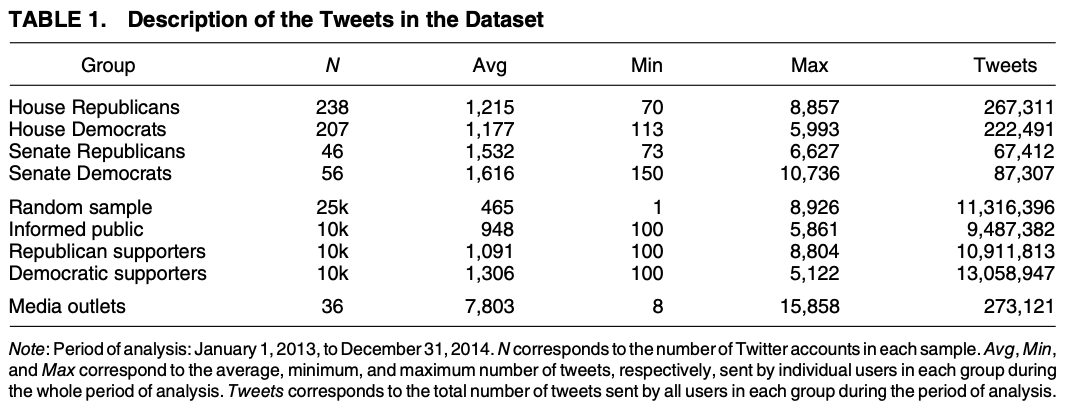
\includegraphics[width=1 \textwidth]{Images/barbera_desc.png}
\end{frame}



\begin{frame}{Barbera et al. (2019): method}
    \begin{itemize}\setlength{\itemsep}{0.8em}
        \item NLP application: how to establish which policy issues are covered by tons of tweets?
        \item Split the aggregated total of tweets sent by each Member of Congress (the \textit{document}) in chunk of $n$-grams (combinations of 1 and 2 words)
        \item Estimate a LDA model to infer topics from the \textit{document}
        \item Fix the number of topics to $K = 100$ and exclude non-political topics (such as celebrations and anniversaries)
        \item Obtain a list of 46 most salient political issues during the 113th Congress
        \item Employ vector autoregression models to explore whose priorities more strongly predict the relationship between citizens and policymakers
    \end{itemize}
\end{frame}

\begin{frame}{}
    \centering
    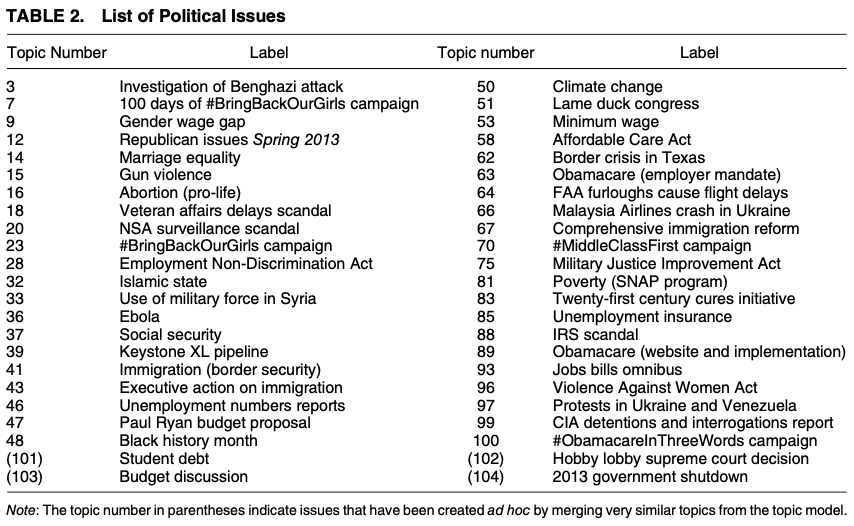
\includegraphics[width=1 \textwidth]{Images/barbera_issues.png}
\end{frame}

\begin{frame}{}
    \centering
    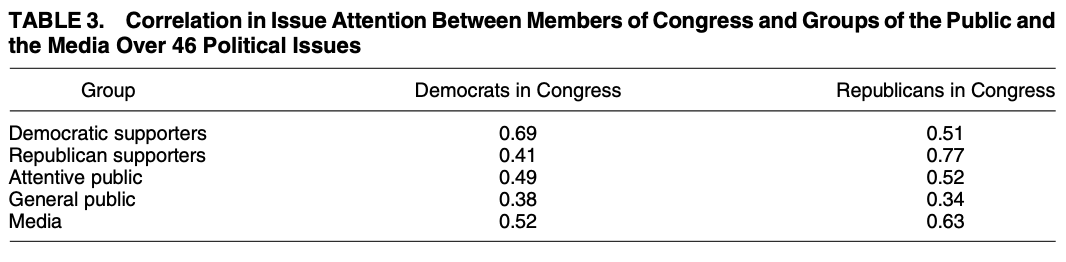
\includegraphics[width=1 \textwidth]{Images/barbera_corr.png}
\end{frame}

\begin{frame}{}
    \centering
    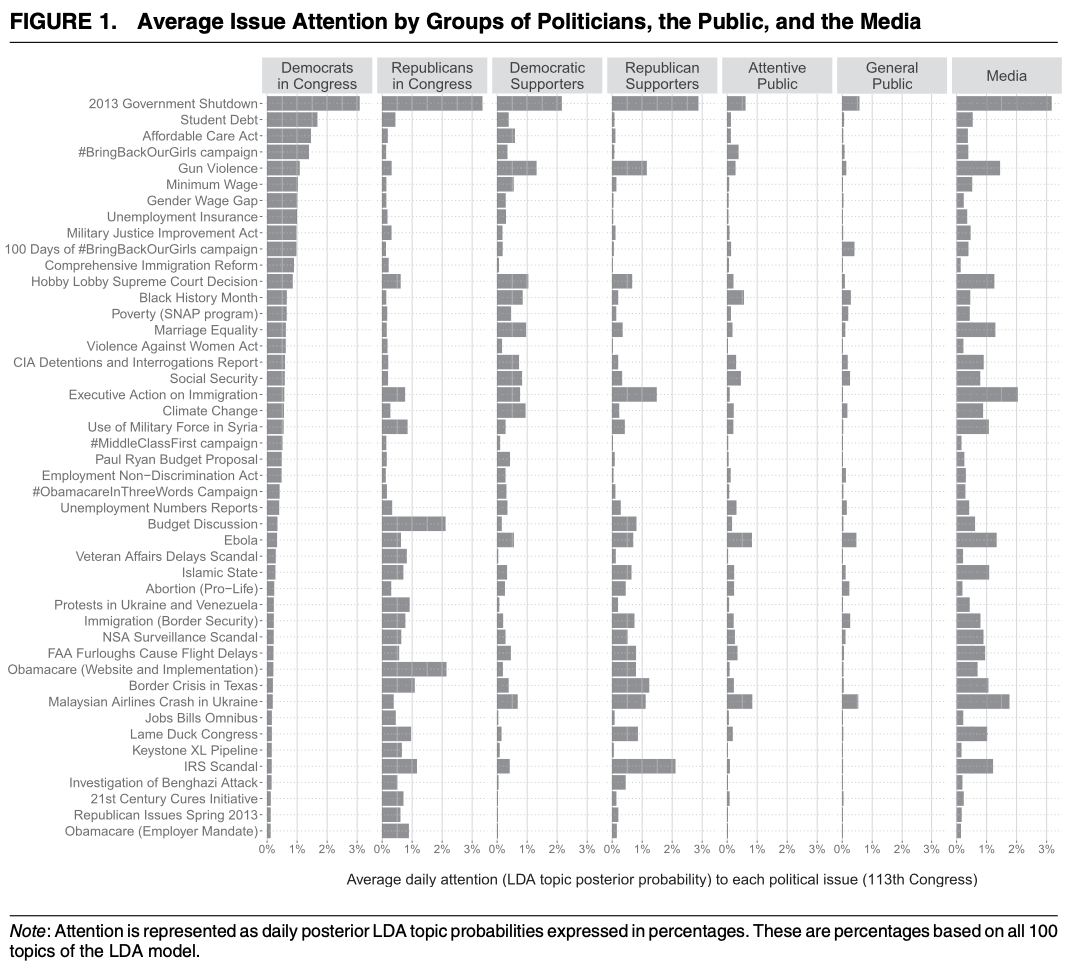
\includegraphics[width=0.8 \textwidth]{Images/barbera_fig1.png}
\end{frame}

\begin{frame}{Barbera et al. (2019): results}
    \begin{itemize}\setlength{\itemsep}{1.2em}
        \item Members of Congress are more likely to follow the issue priorities of the public than to lead them
        \item Lawmakers more likely to change their behaviour after shifts in attention by party supporters
        \item Less likely to be responsive to the general public
        \item Mass media more likely to cover issues of interest to partisans for commercial reasons
    \end{itemize}
\end{frame}

\begin{frame}{}
    \centering
    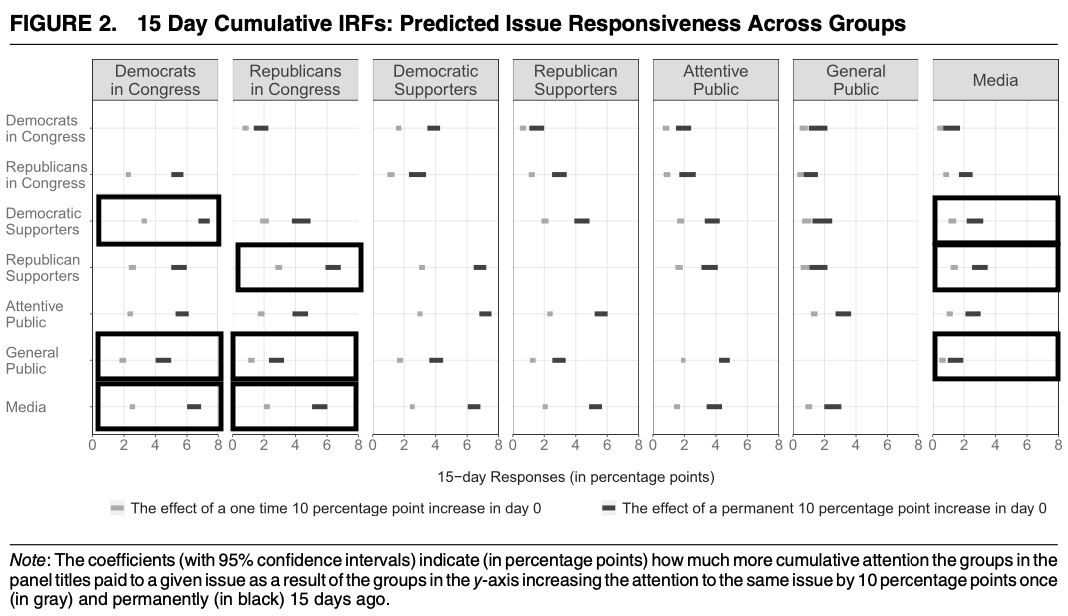
\includegraphics[width=1 \textwidth]{Images/barbera_mainres.png}
\end{frame}

\begin{frame}{Zooming in}
    \centering
    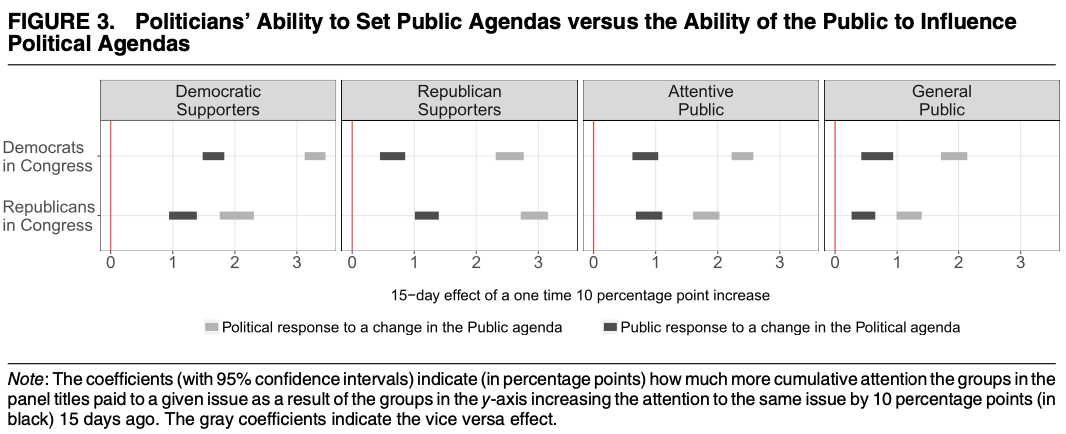
\includegraphics[width=1 \textwidth]{Images/barbera_mainres2.png}
\end{frame}

\begin{frame}{}
        \centering
    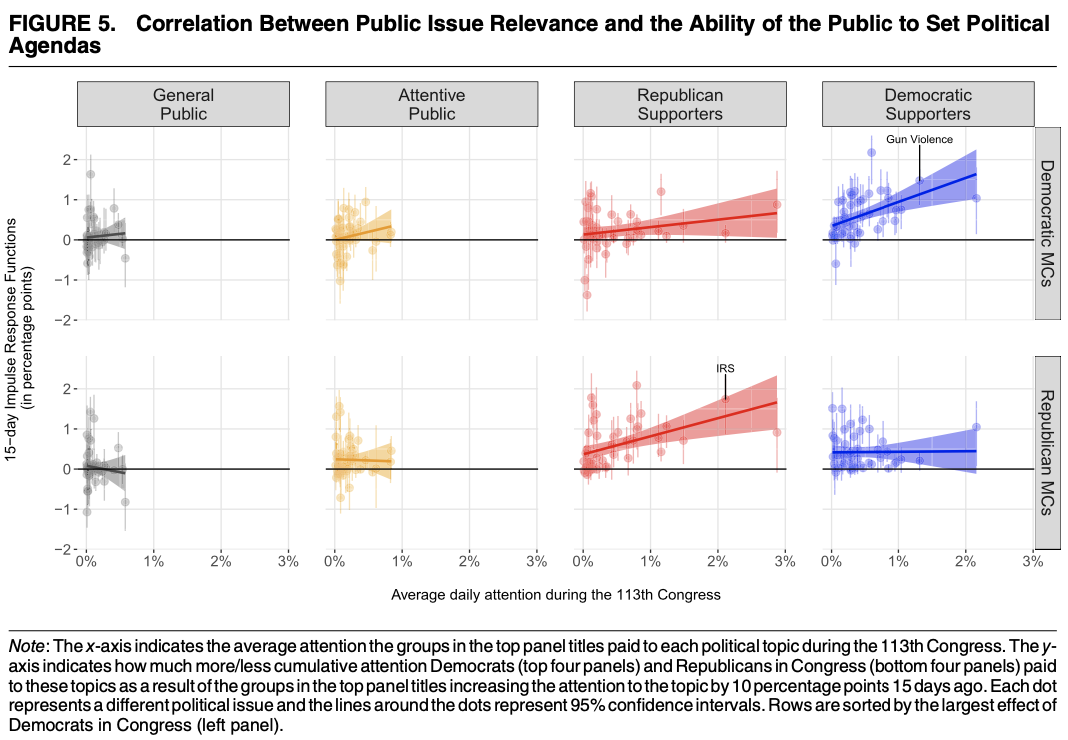
\includegraphics[width=1 \textwidth]{Images/barbera_res3.png}
\end{frame}

\begin{frame}{}
        \centering
    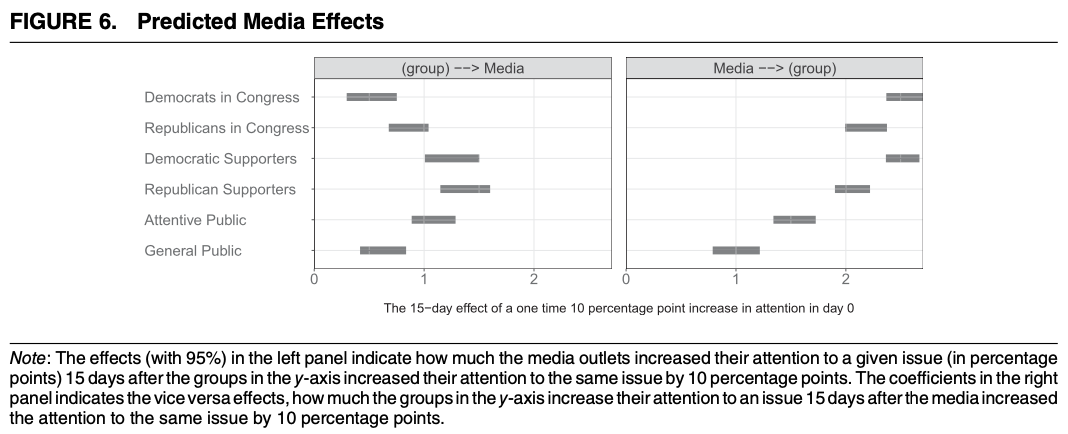
\includegraphics[width=1 \textwidth]{Images/barbera_mediaeff.png}
\end{frame}

\begin{frame}{Barbera et al. (2019): discussion}
\begin{itemize}\setlength{\itemsep}{1.2em}
    \item Mechanisms found in the paper reinforce polarization
    \item Possible directions for future research:
    \begin{itemize}\setlength{\itemsep}{1.2em}\vspace{5pt}
        \item Is the President able to set his own political agenda?
        \item Do politicians running in safe vs. competitive districts respond to different types of constituents?
        \item Do politicians respond differently to constituents' issue priorities depending on the issues they own?
        \item How would these results differ across institutional or political contexts?
    \end{itemize}
\end{itemize}
    
\end{frame}


\end{document}
